%Title of section
\section{基于动态伸缩的容器调度策略}

\subsection{问题定义}

\begin{frame}
\frametitle{问题定义}
\framesubtitle{调度目标}
\begin{itemize}
    \item 最小化CaaS数据中心总能耗
    \begin{equation}
    \begin{align*}
            &\min\quad P_{dc}(t)=\sum_{i=1}^{N_s} P_i(t) \\
            &s.t.\quad
            \begin{cases}
            \sum_{j=1}^{N_{vm}}vm_{(j,i,r)}(t) < S_(i,r),\\
            \forall i \in [1,N_s],\ \forall r \in \{CPU,Memory,Disk,BW\} \\
            \\
            \sum_{k=1}^{N_{c}}c_{(k,j,i,r)}(t) < vm_(j,i,r),\\
            \forall i \in [1,N_{vm}],\ \forall r \in \{CPU,Memory,Disk,BW\}
            \end{cases}
    \end{align*}
    \end{equation}
\end{itemize}
\end{frame}

\subsection{系统结构}

\begin{frame}
\frametitle{系统结构}
\framesubtitle{调度系统模型}
\begin{exampleblock}{调度系统模型设计思路}
\begin{itemize}
    \item 主机状态模块:标记高负载/低负载主机
    \begin{itemize}
            \item 高负载主机列表
            \item 低负载主机列表
    \end{itemize}
    \item 容器状态模块
    \begin{itemize}
        \item 负载预测结果与调整阈值 $\Rightarrow$ 计算容器扩容、缩容数量
        \item 从高负载主机列表中选择需要迁移容器
    \end{itemize}
    \item 容器调度模块
     \begin{itemize}
             \item 为待迁移容器找到目的地
             \item 基于资源约束条件合并低负载主机上的容器
             \item 销毁并关闭空载的虚拟机和服务器 $\Rightarrow$ 避免不必要的能耗
     \end{itemize}
\end{itemize}
\end{exampleblock}
\end{frame}

\begin{frame}
\frametitle{系统结构}
\framesubtitle{调度系统示意图}
\begin{figure}[htb]
    \centering
    \includegraphics[width=0.5\textwidth]{figures/fig14_scheduler_sys.jpg}
    \caption{基于动态伸缩的容器调度系统结构}
    \label{fig:fig14}
\end{figure}
\bigskip
\end{frame}

\subsection{调度算法}

\begin{frame}
\frametitle{调度算法}
\framesubtitle{主机状态模块(1/1):主机状态标记算法 - 标记主机状态}
\begin{itemize}
    \item 主机状态标记:通过\textbf{静态阈值法}设置$T_{ol}$和$T_{ul}$
    \begin{equation}
        Host\ status =
        \begin{cases}
            \textbf{Over-Load} \ \ \ if \ U_i(t) > T_{ol} \\
            \textbf{Under-Load} \ \ if\ U_i(t) < T_{ul}
        \end{cases}
    \end{equation}
\end{itemize}
\end{frame}

\begin{frame}
\frametitle{调度算法}
\framesubtitle{容器状态模块(1/2):容器伸缩算法 - 计算容器扩缩容数量}
\begin{itemize}
    \item 令应用$V$的当前容器副本总数$n=n_{now}$
    \begin{itemize}
        \item 应用$V$负载上界:$L_v^u = \sum_{i=1}^{n_{now}}l_i^u$
        \item 应用$V$负载下界:$L_v^l = \sum_{i=1}^{n_{now}}l_i^l$
    \end{itemize}
    \item 设置用于应用$V$扩缩容的调整阈值为$L_v$
        \begin{itemize}
            \item 满足公式\ref{eq:lu}(负载落在$L_v$之上) $\Rightarrow$ 扩容 $\lceil \frac{(L_v^u+L_v^l)}{2L_v} - n_{now} \rceil$ 个
            \item 满足公式\ref{eq:ll}(负载落在$L_v$之下)  $\Rightarrow$ 缩容$\lceil n_{now} - \frac{(L_v^u+L_v^l)}{2L_v} {\color{red} - 1}\rceil$ 个
        \end{itemize}
    \begin{equation}
        \frac{L_v^u - n_{now} \times L_v}{n_{now} \times L_v - L^l_v} > 1
        \label{eq:lu}
    \end{equation}
    \begin{equation}
        \frac{(n_{now} - 1) \times L_v - L_v^l}{L_v^u - (n_{now} - 1) \times L_v} > 1
        \label{eq:ll}
    \end{equation}
\end{itemize}
\end{frame}

\begin{frame}
\frametitle{调度算法}
\framesubtitle{容器状态模块(2/2):容器选择算法 - 选择高负载主机上需要迁移容器}
\begin{figure}[htb]
    \centering
    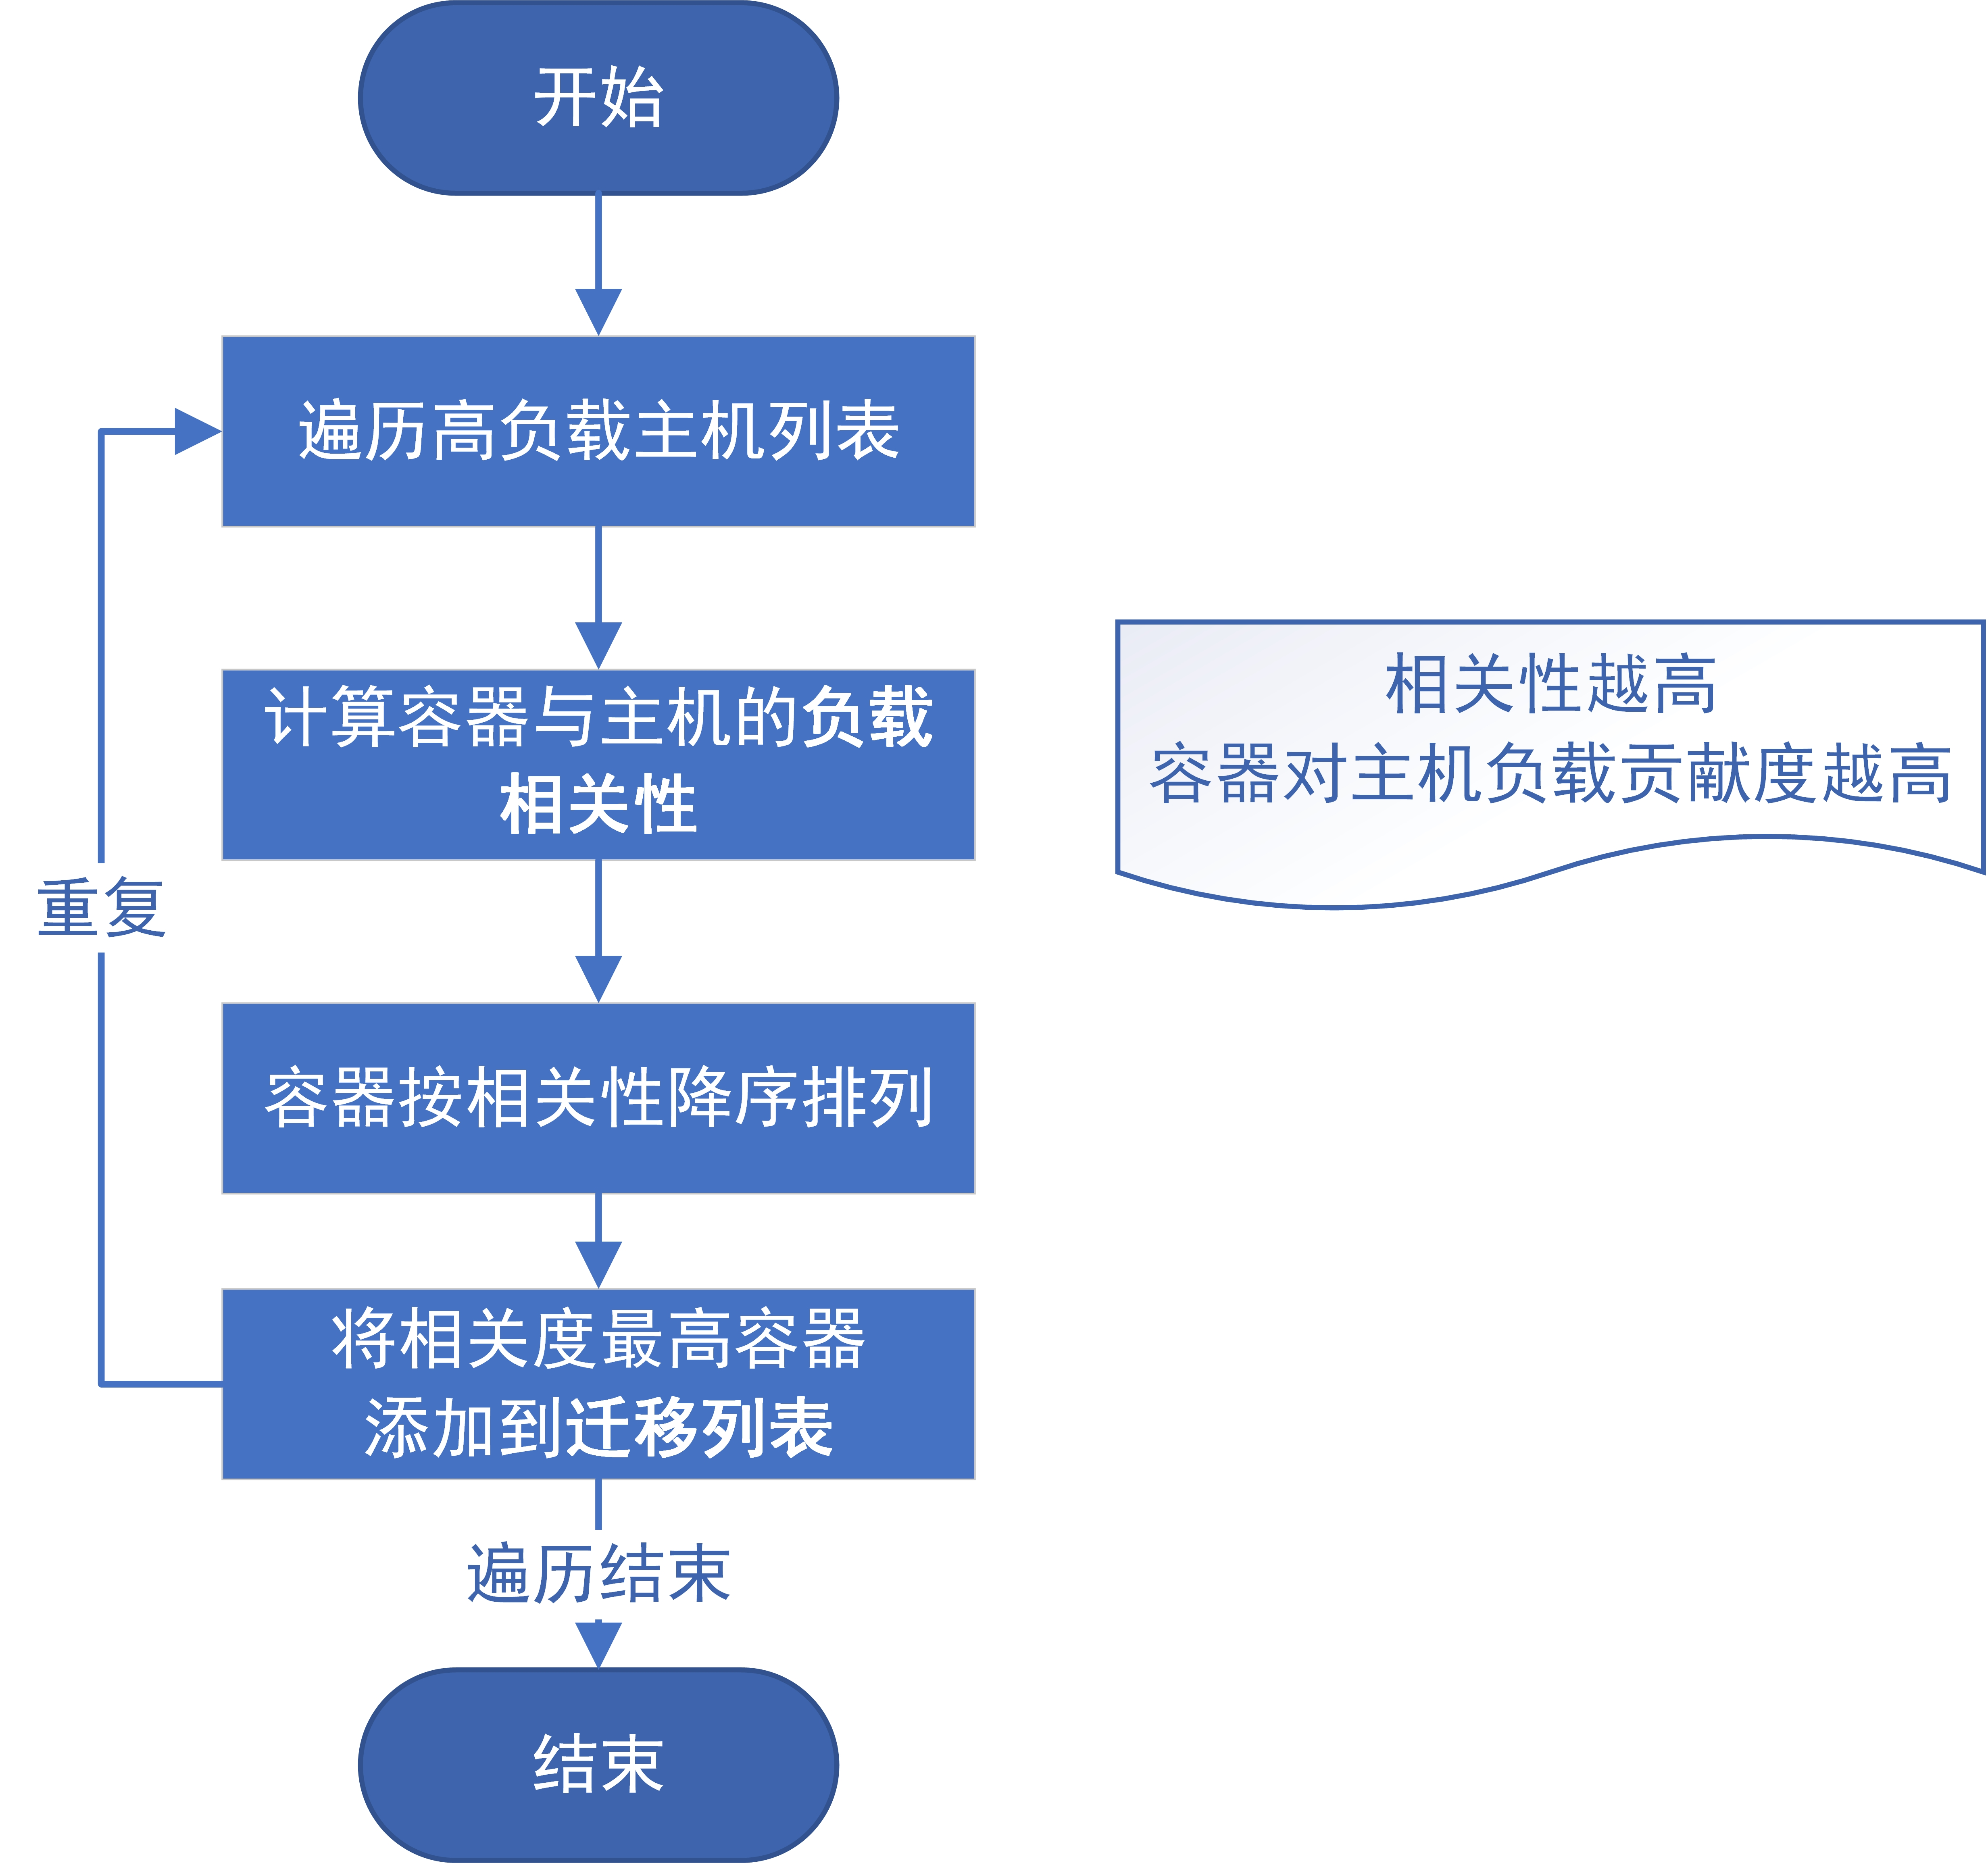
\includegraphics[width=0.52\textwidth]{figures/fig_4_1.jpg}
    \caption{容器选择算法流程}
    \label{fig:fig_4_1}
\end{figure}
\bigskip
\end{frame}

\begin{frame}
\frametitle{调度算法}
\framesubtitle{容器调度模块(1/3):主机选择算法 - 选择容器迁移目的主机}
\begin{figure}[htb]
    \centering
    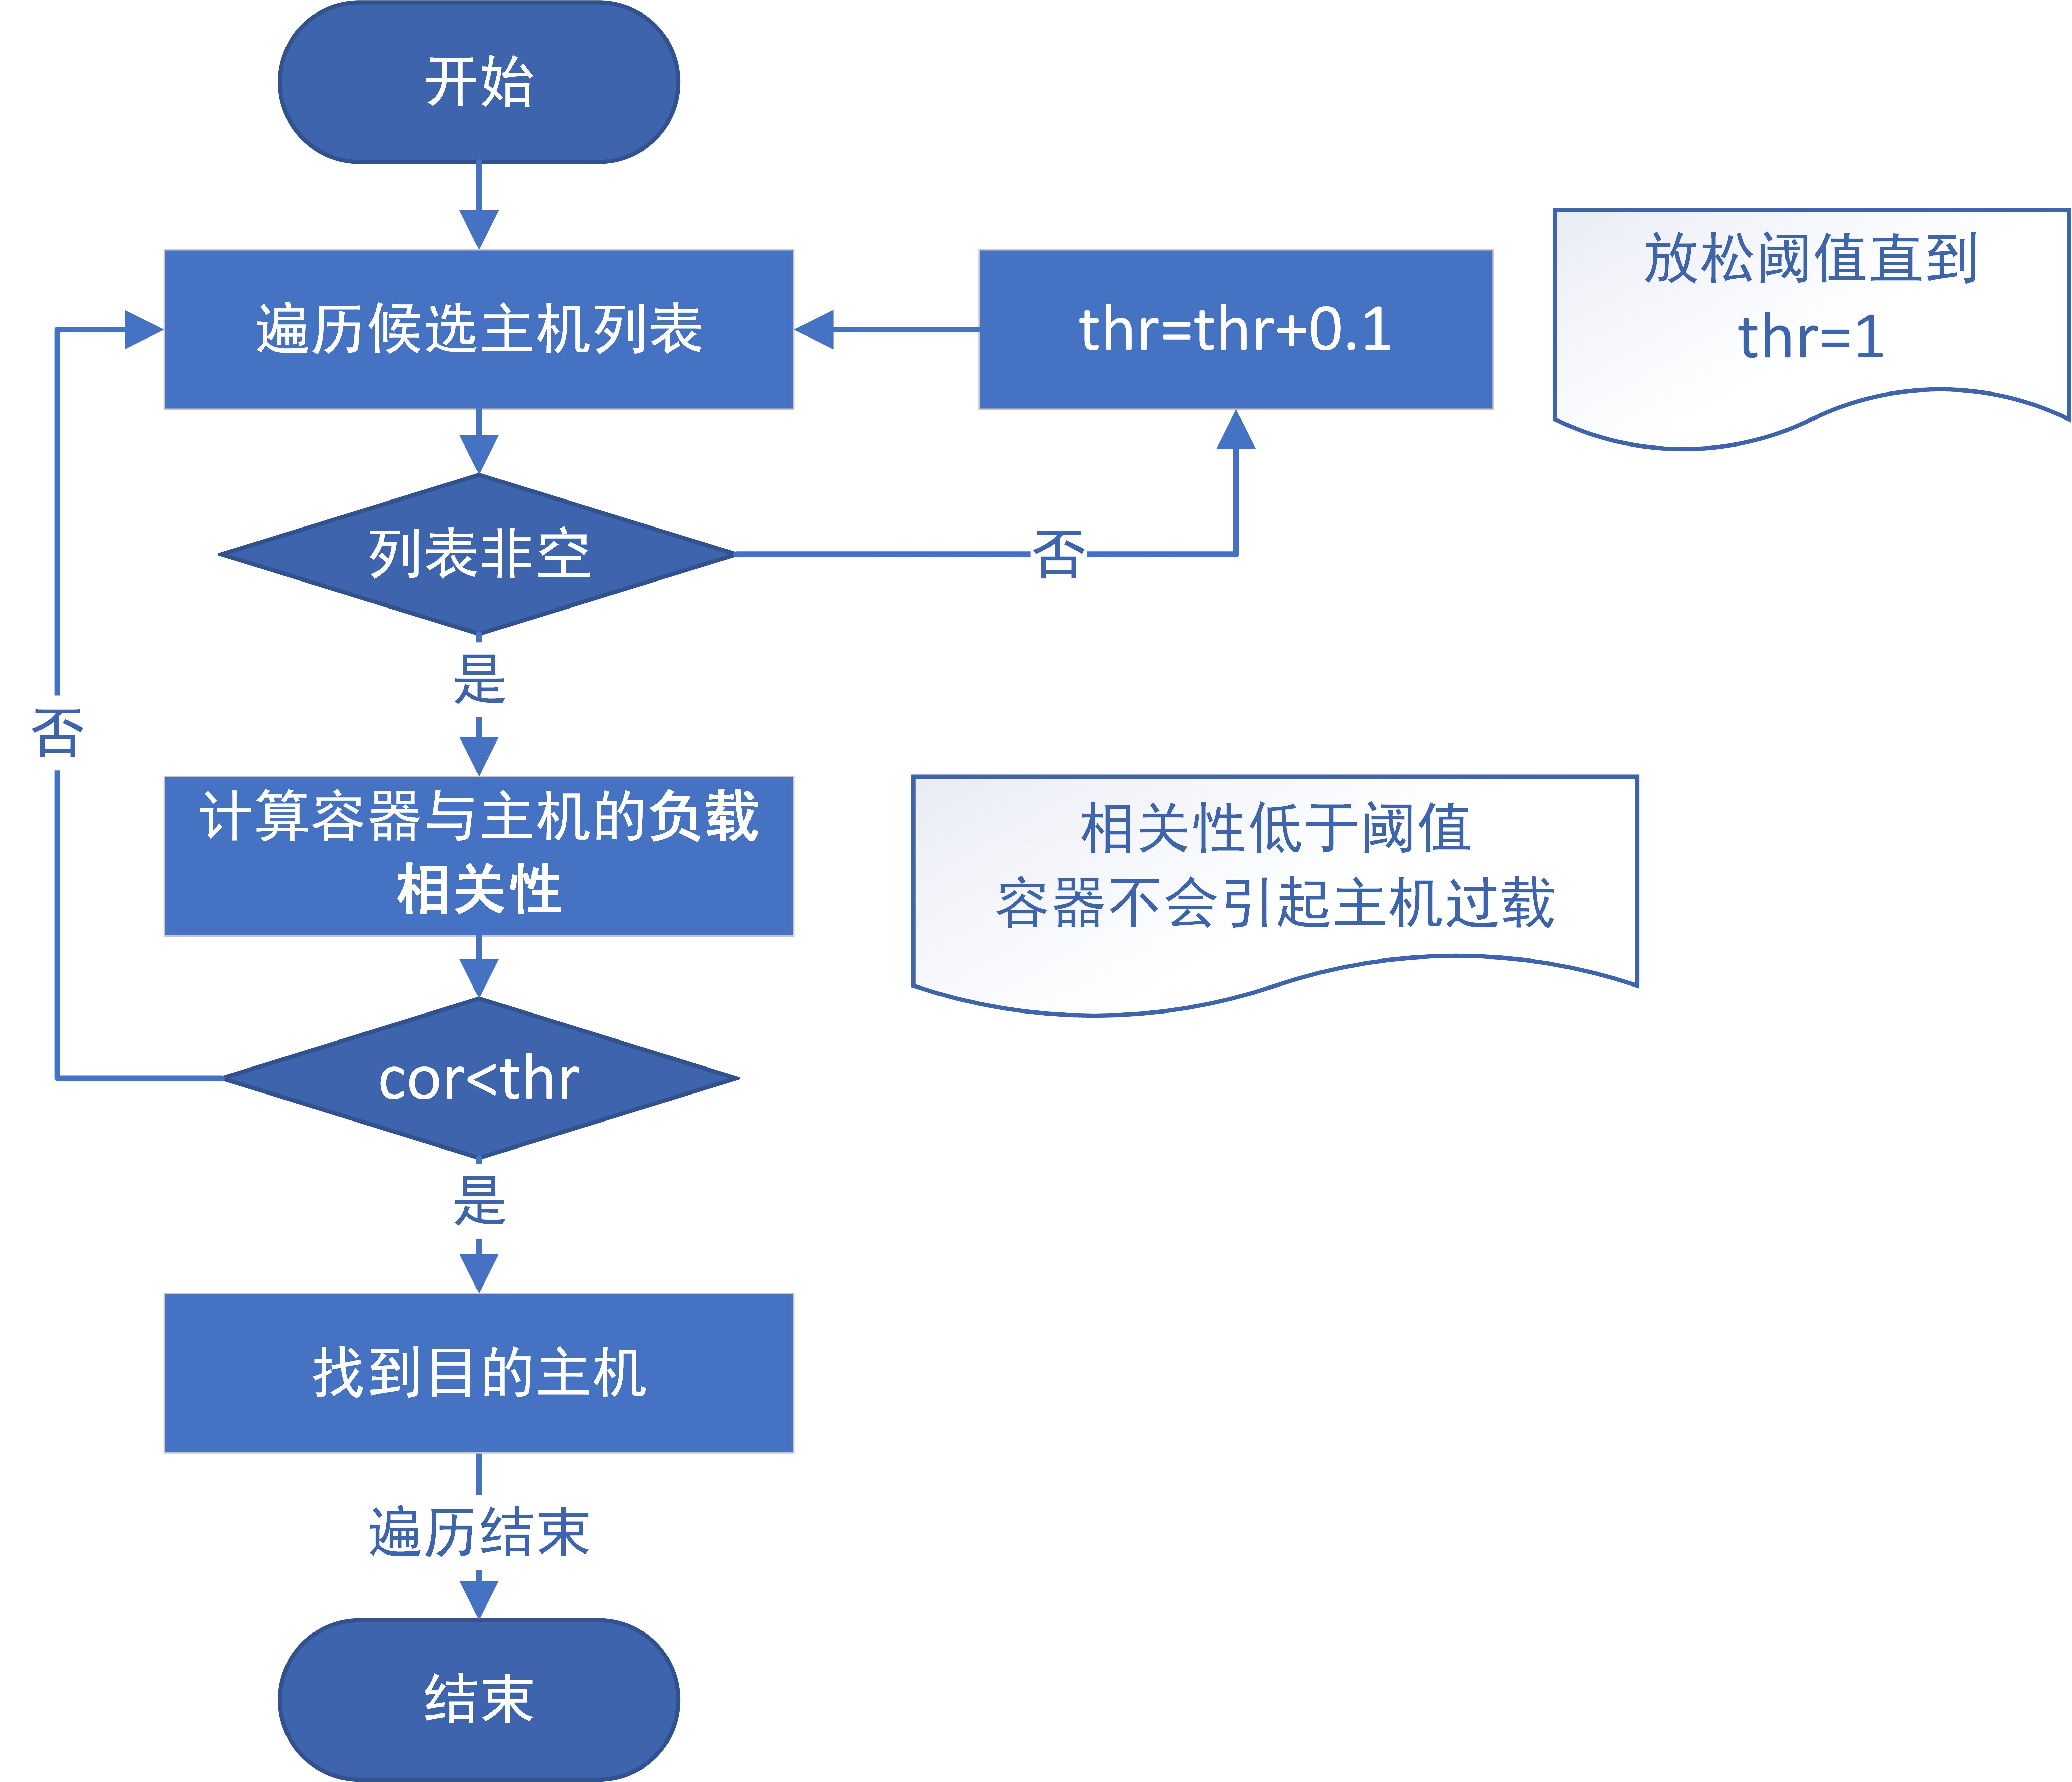
\includegraphics[width=0.58\textwidth]{figures/fig_4_2.jpg}
    \caption{主机选择算法流程}
    \label{fig:fig_4_2}
\end{figure}
\bigskip
\end{frame}

\begin{frame}
\frametitle{调度算法}
\framesubtitle{容器调度模块(2/3):容器迁移和放置算法 - 迁移高负载主机上容器、放置新增容器}
\begin{figure}[htb]
    \centering
    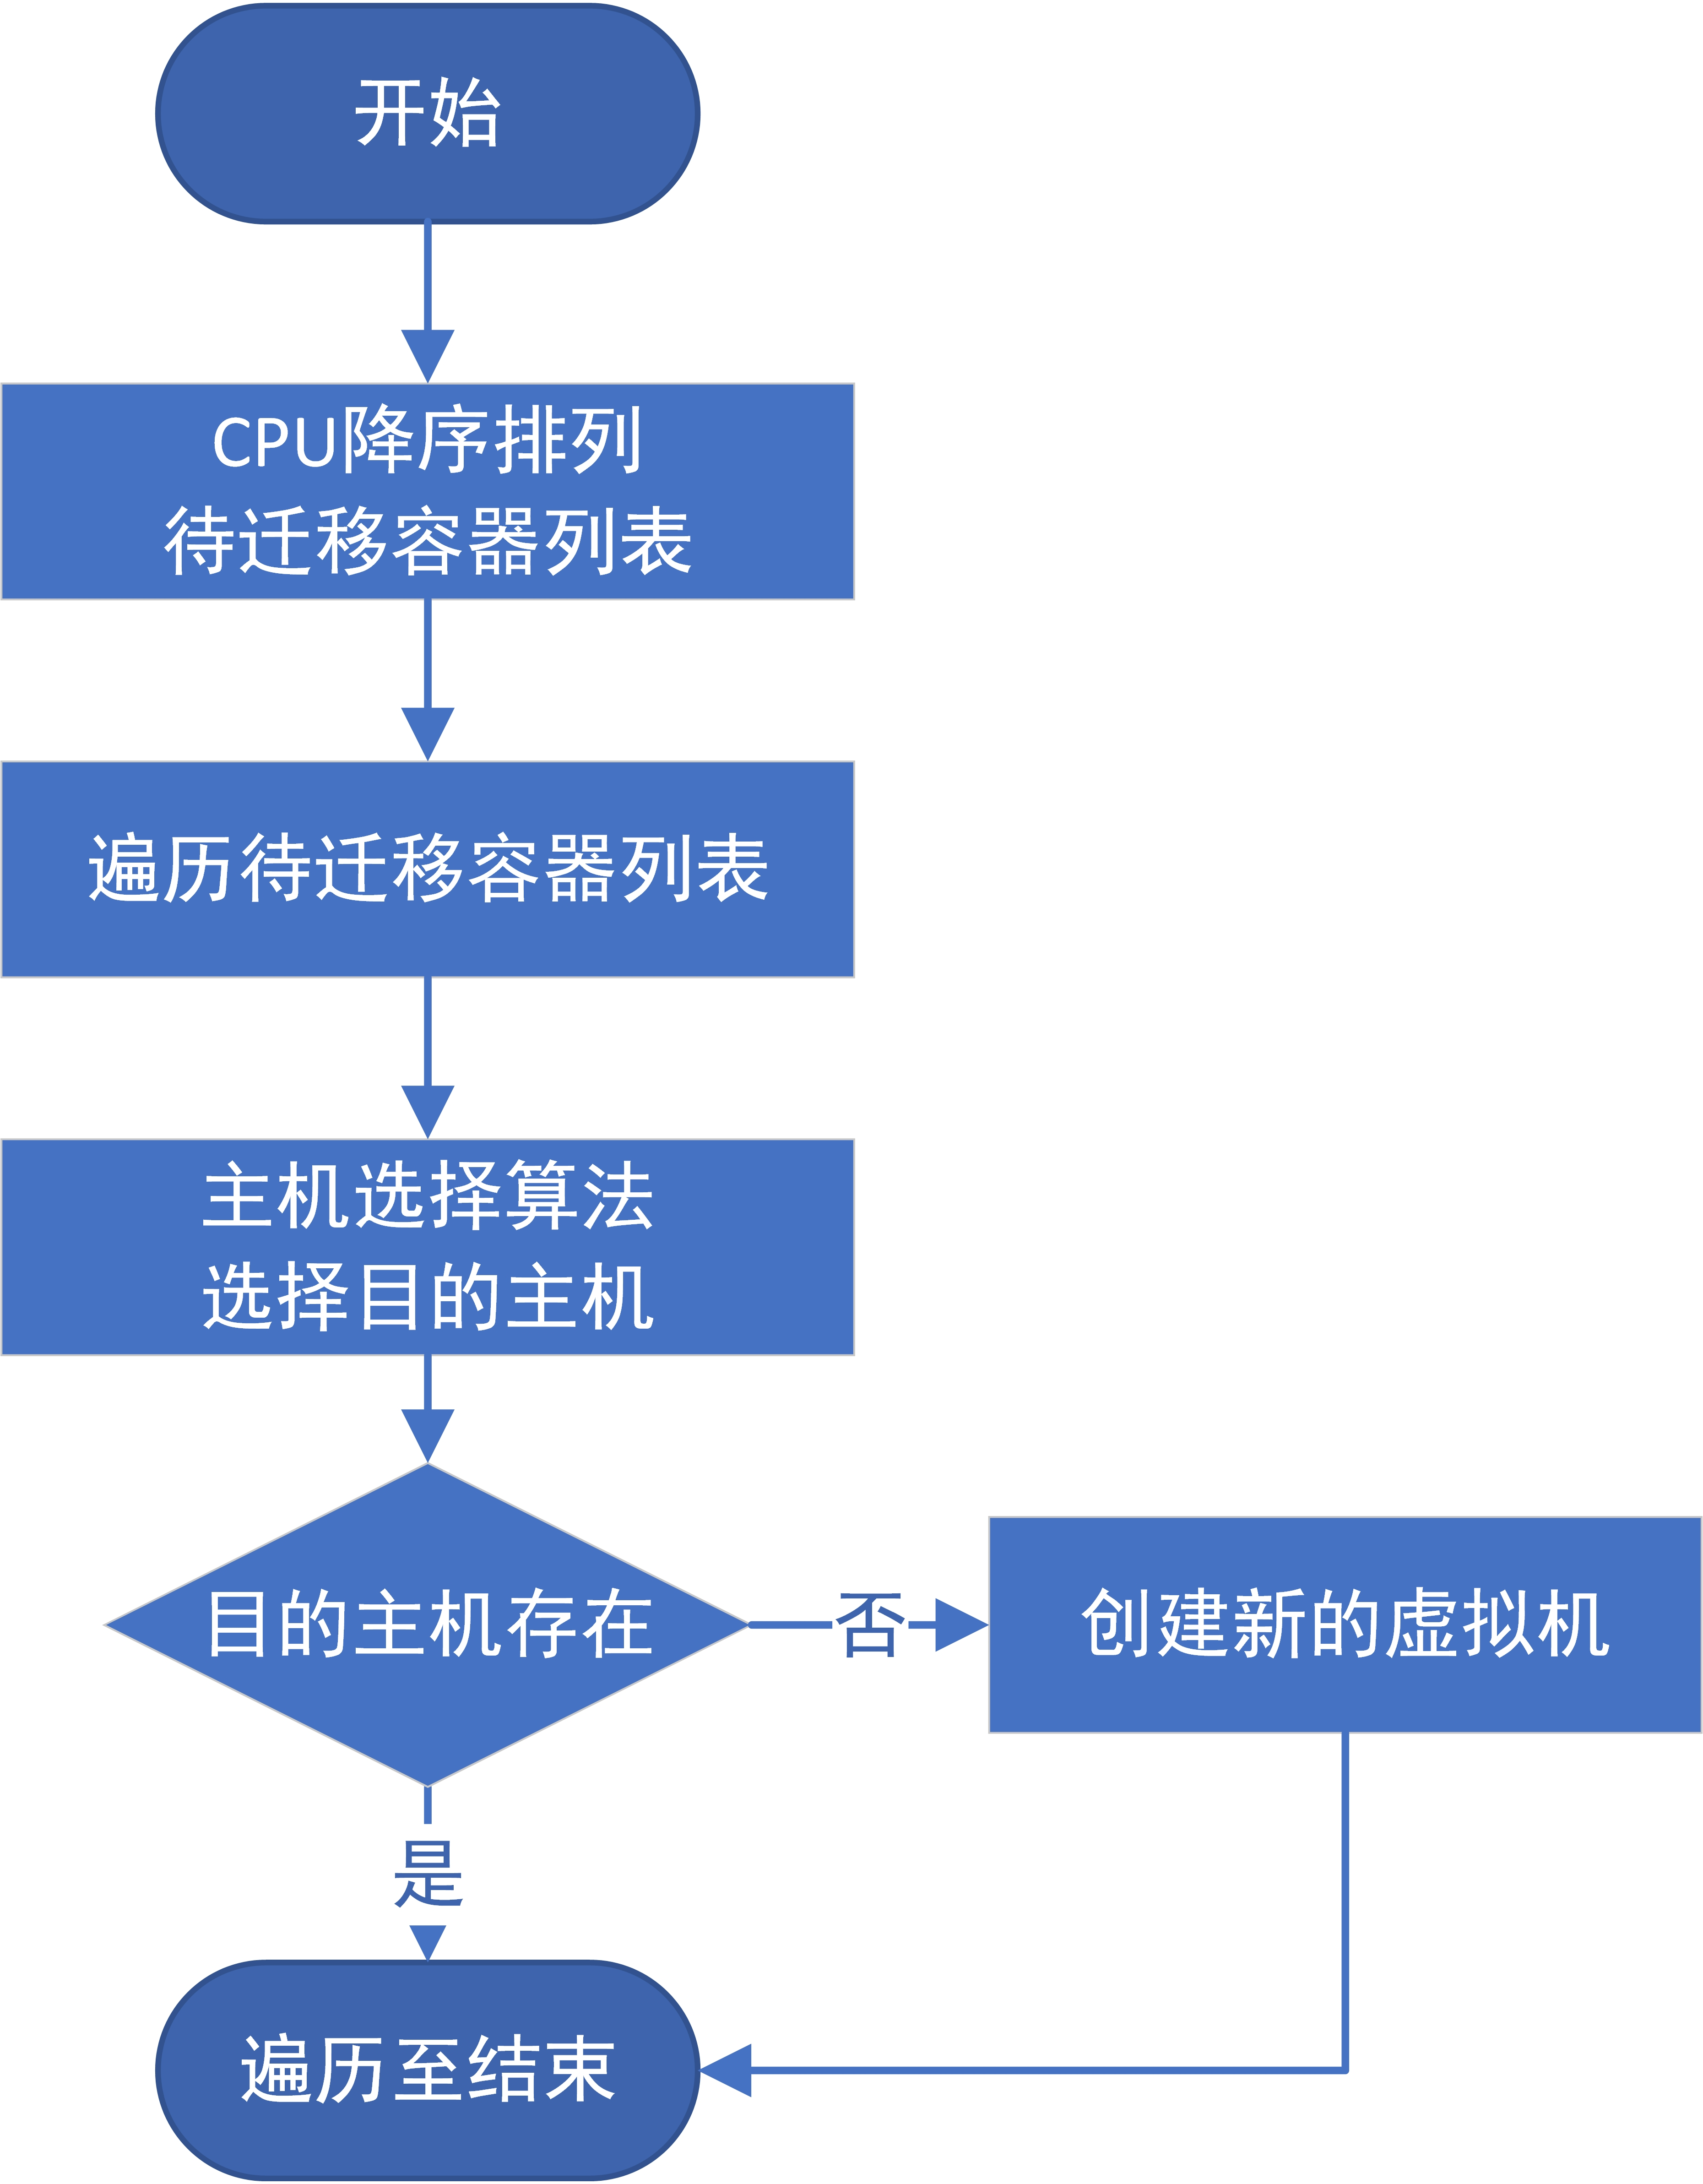
\includegraphics[width=0.4\textwidth]{figures/fig_4_3.jpg}
    \caption{容器迁移和放置算法流程}
    \label{fig:fig_4_3}
\end{figure}
\end{frame}

\begin{frame}
\frametitle{调度算法}
\framesubtitle{容器调度模块(3/3):容器合并算法 - 合并低负载主机容器}
\begin{figure}[htb]
    \centering
    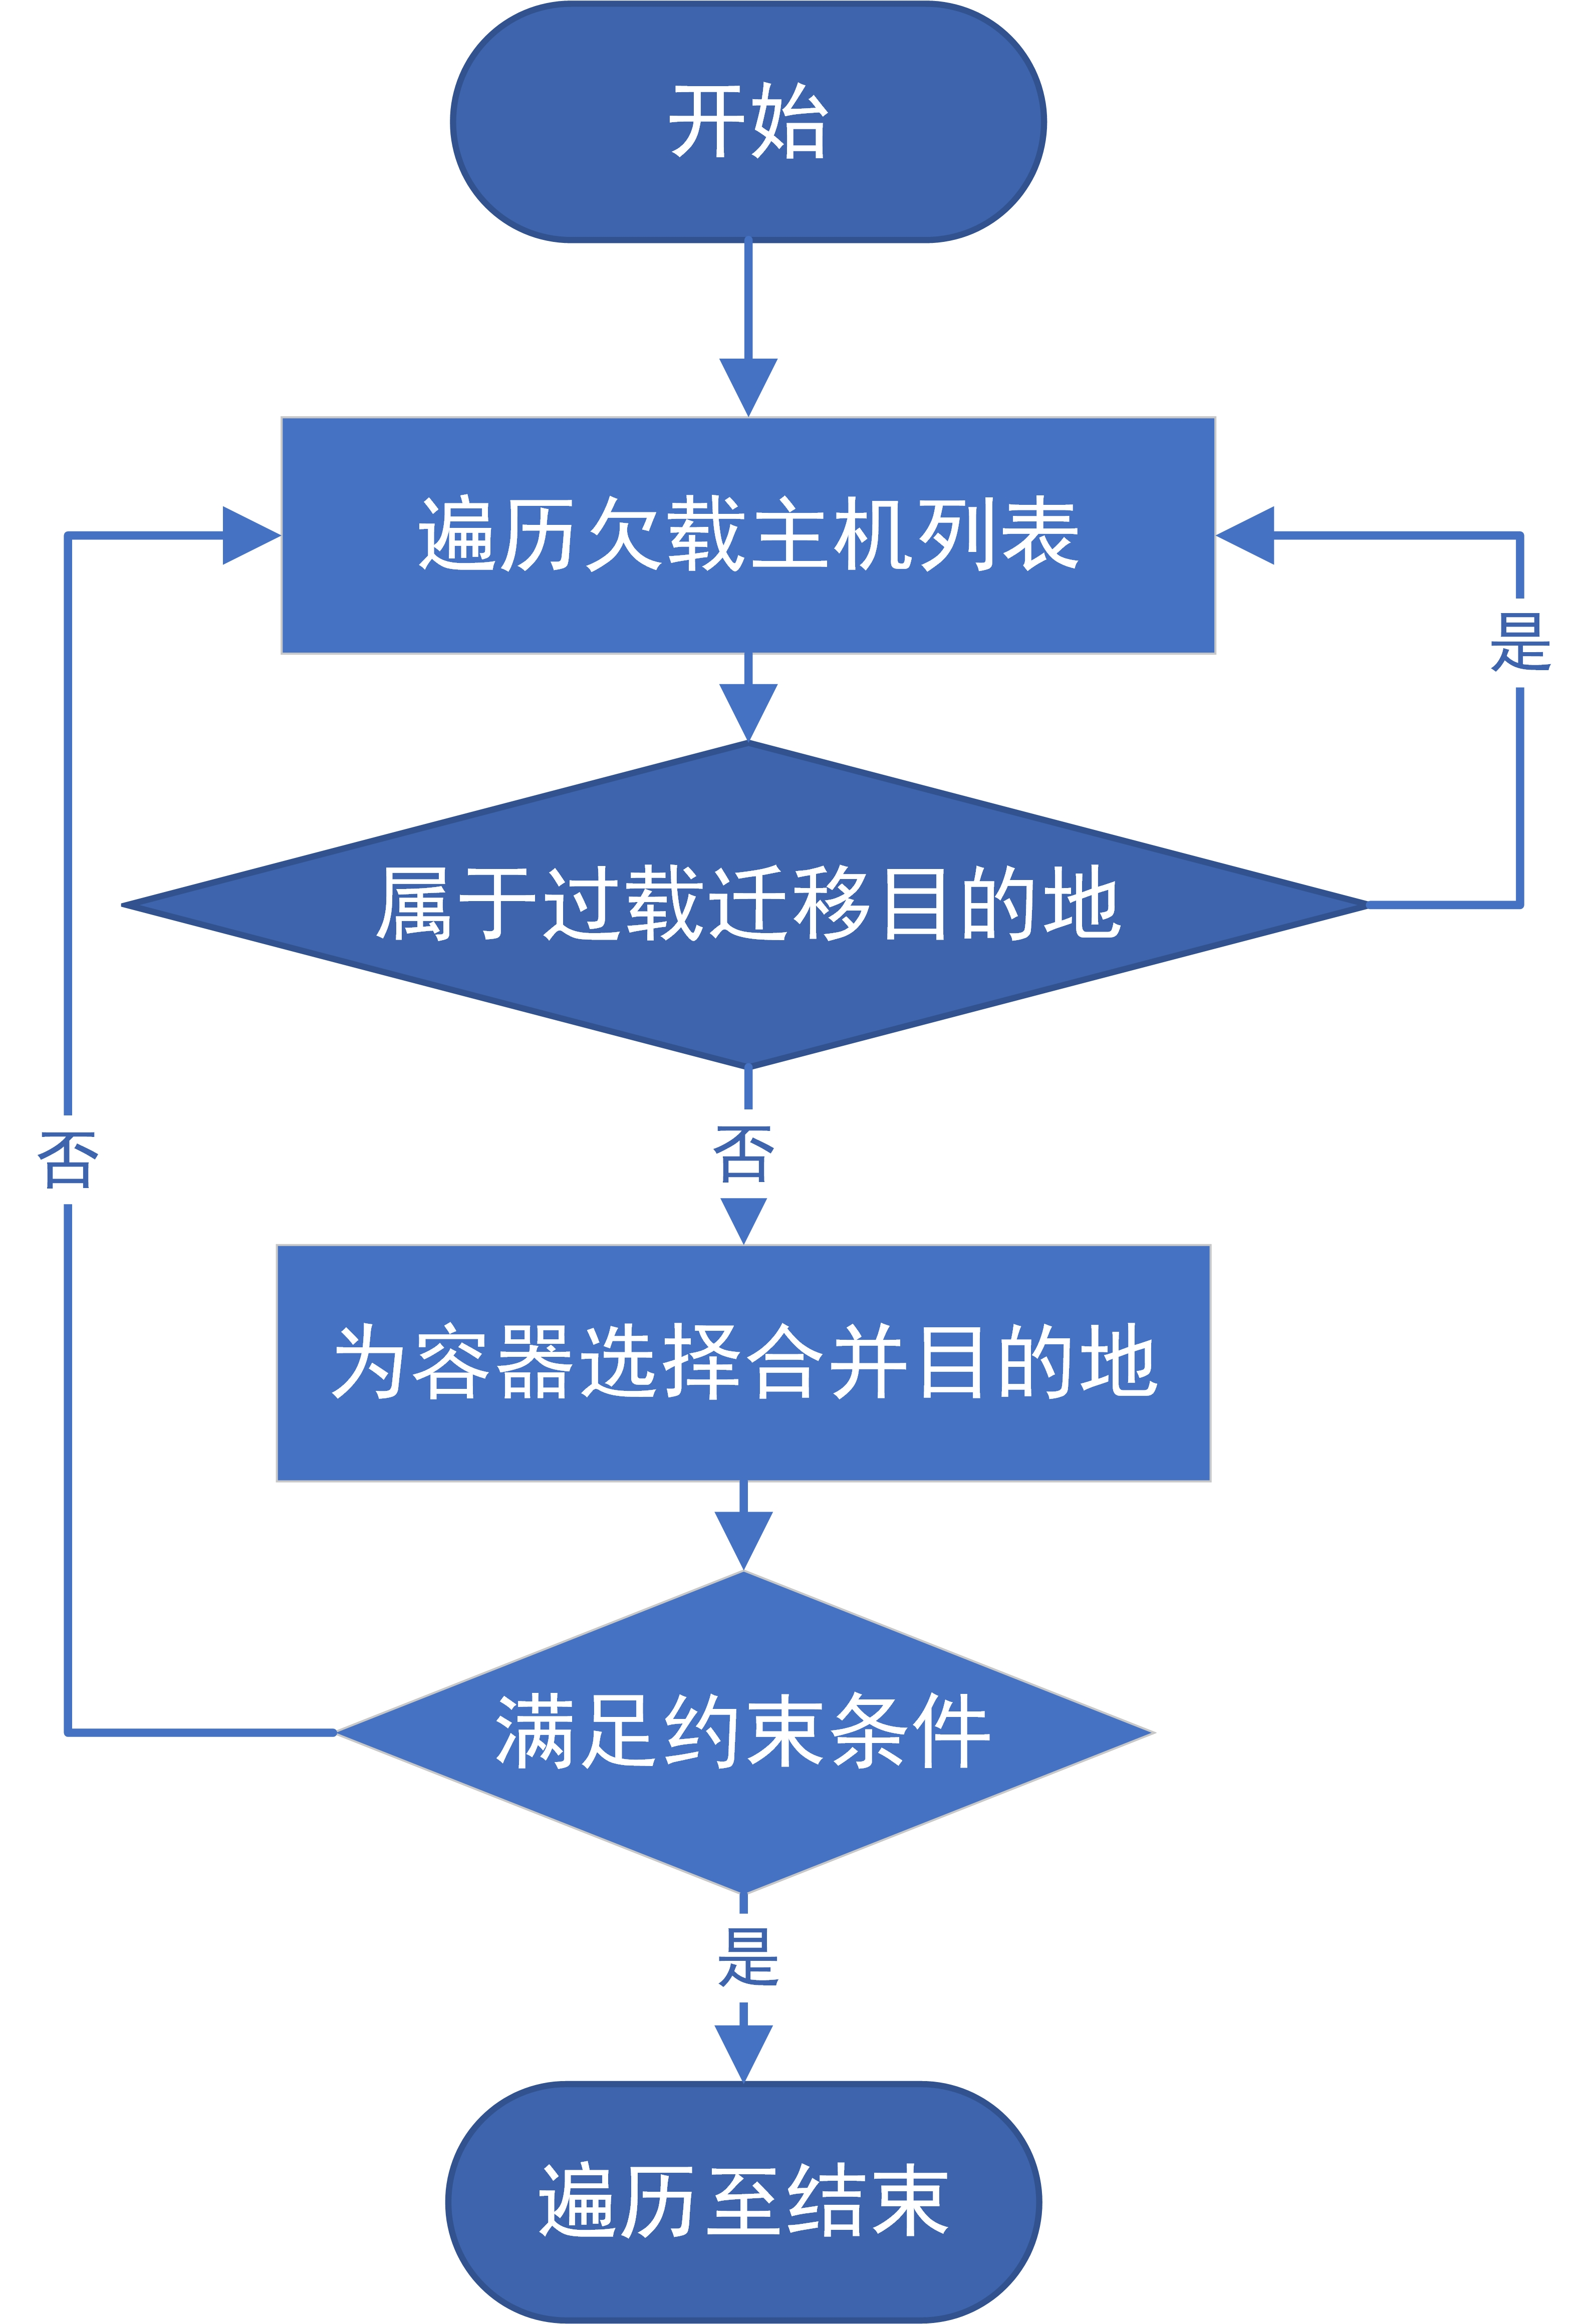
\includegraphics[width=0.36\textwidth]{figures/fig_4_4.jpg}
    \caption{容器合并算法流程}
    \label{fig:fig_4_4}
\end{figure}
\end{frame}

\subsection{实验结果与分析}

\begin{frame}
\frametitle{实验结果与分析}
\framesubtitle{QoS指标}
\begin{itemize}
    \item SLA违反率:容器未分配的CPU资源量在总请求量中的占比
    \begin{equation}
    \begin{align*}
        &SLA = \sum_{i=1}^{N_s}\sum_{j=1}^{N_{vm}}\sum_{p=1}^{N_v}
        \frac{CPU_r(vm_{ji},t_p) - CPU_a(vm_{ji},t_p)}{CPU_r(vm_{ji},t_p)} \\
        &\begin{cases}
            CPU_r(vm_{ji},t_p) = \sum_{k=1}^{N_c^{ji}}CPU_r(c_{kji},t_p) \\
            CPU_a(vm_{ji},t_p) = \sum_{k=1}^{N_c^{ji}}CPU_a(c_{kji},t_p)
        \end{cases}
    \end{align*}
    \end{equation}
    \item 容器对CPU资源的请求量:依据\textbf{超量因子}$P_n$从历史记录中获取
        \begin{enumerate}
            \item 从容器负载历史记录中选择一个负载值 $L_{per}$
            \item 概率 $P(L \le L_{per}) \ge P_n$
            \item $min(L_{per})$ 即为容器对CPU资源的请求量
        \end{enumerate}
\end{itemize}
\end{frame}

\begin{frame}
\frametitle{实验结果与分析}
\framesubtitle{实验设置}
\begin{itemize}
    \item 容器负载数据(PlanetLab)、服务器和虚拟机配置、CloudSim
    \item 对比算法
    \begin{itemize}
        \item \textbf{FFHS(Kubernetes)}:选择第一台满足资源请求的主机
        \item \textbf{LFHS}:FFHS基础上增加主机CPU降序排列预处理
        \item \textbf{WEEC}:聚类划分容器,基于能耗特征的启发式算法
        \item \textbf{本文基于动态伸缩的容器调度策略}
    \end{itemize}
    \item 对照实验:
    \begin{itemize}
        \item 控制容器伸缩的\textbf{"应用总体负载阈值"$=70\%$}
        \item CorHS中的\textbf{"负载相关度阈值"$=0.5$}
    \end{itemize}
    \begin{table}[hftb]
        \centering
        \resizebox{0.8\textwidth}{!}{%
            \begin{tabular}{ccccc}
                \toprule
                \textbf{实验组} & \textbf{约束目标} & \textbf{UL} & \textbf{OL} & \textbf{Overbooking}\\
                \midrule
                group.1 & OL阈值 & $70\%$ & $[80\%,90\%,100\%]$ & $80th$\\
                group.2 & UL阈值 & $[50\%,60\%,70\%]$ & $80\%$ & $80th$ \\
                group.3 & Overbooking阈值& $70\%$ & $80\%$ & $[20th,40th,80th]$\\
                \bottomrule
            \end{tabular}
        }
        \caption{实验对照组设置}
        \label{tab:tab5}
    \end{table}
\end{itemize}
\end{frame}

\begin{frame}
\frametitle{实验结果与分析}
\framesubtitle{实验结果:group.1 \textbf{UL=$70\%$ OL=$[80\%,90\%,100\%]$, Overbooking=$80th$}}
\begin{minipage}{\textwidth}
    \centering
    \begin{figure}[htb]
    \centering
    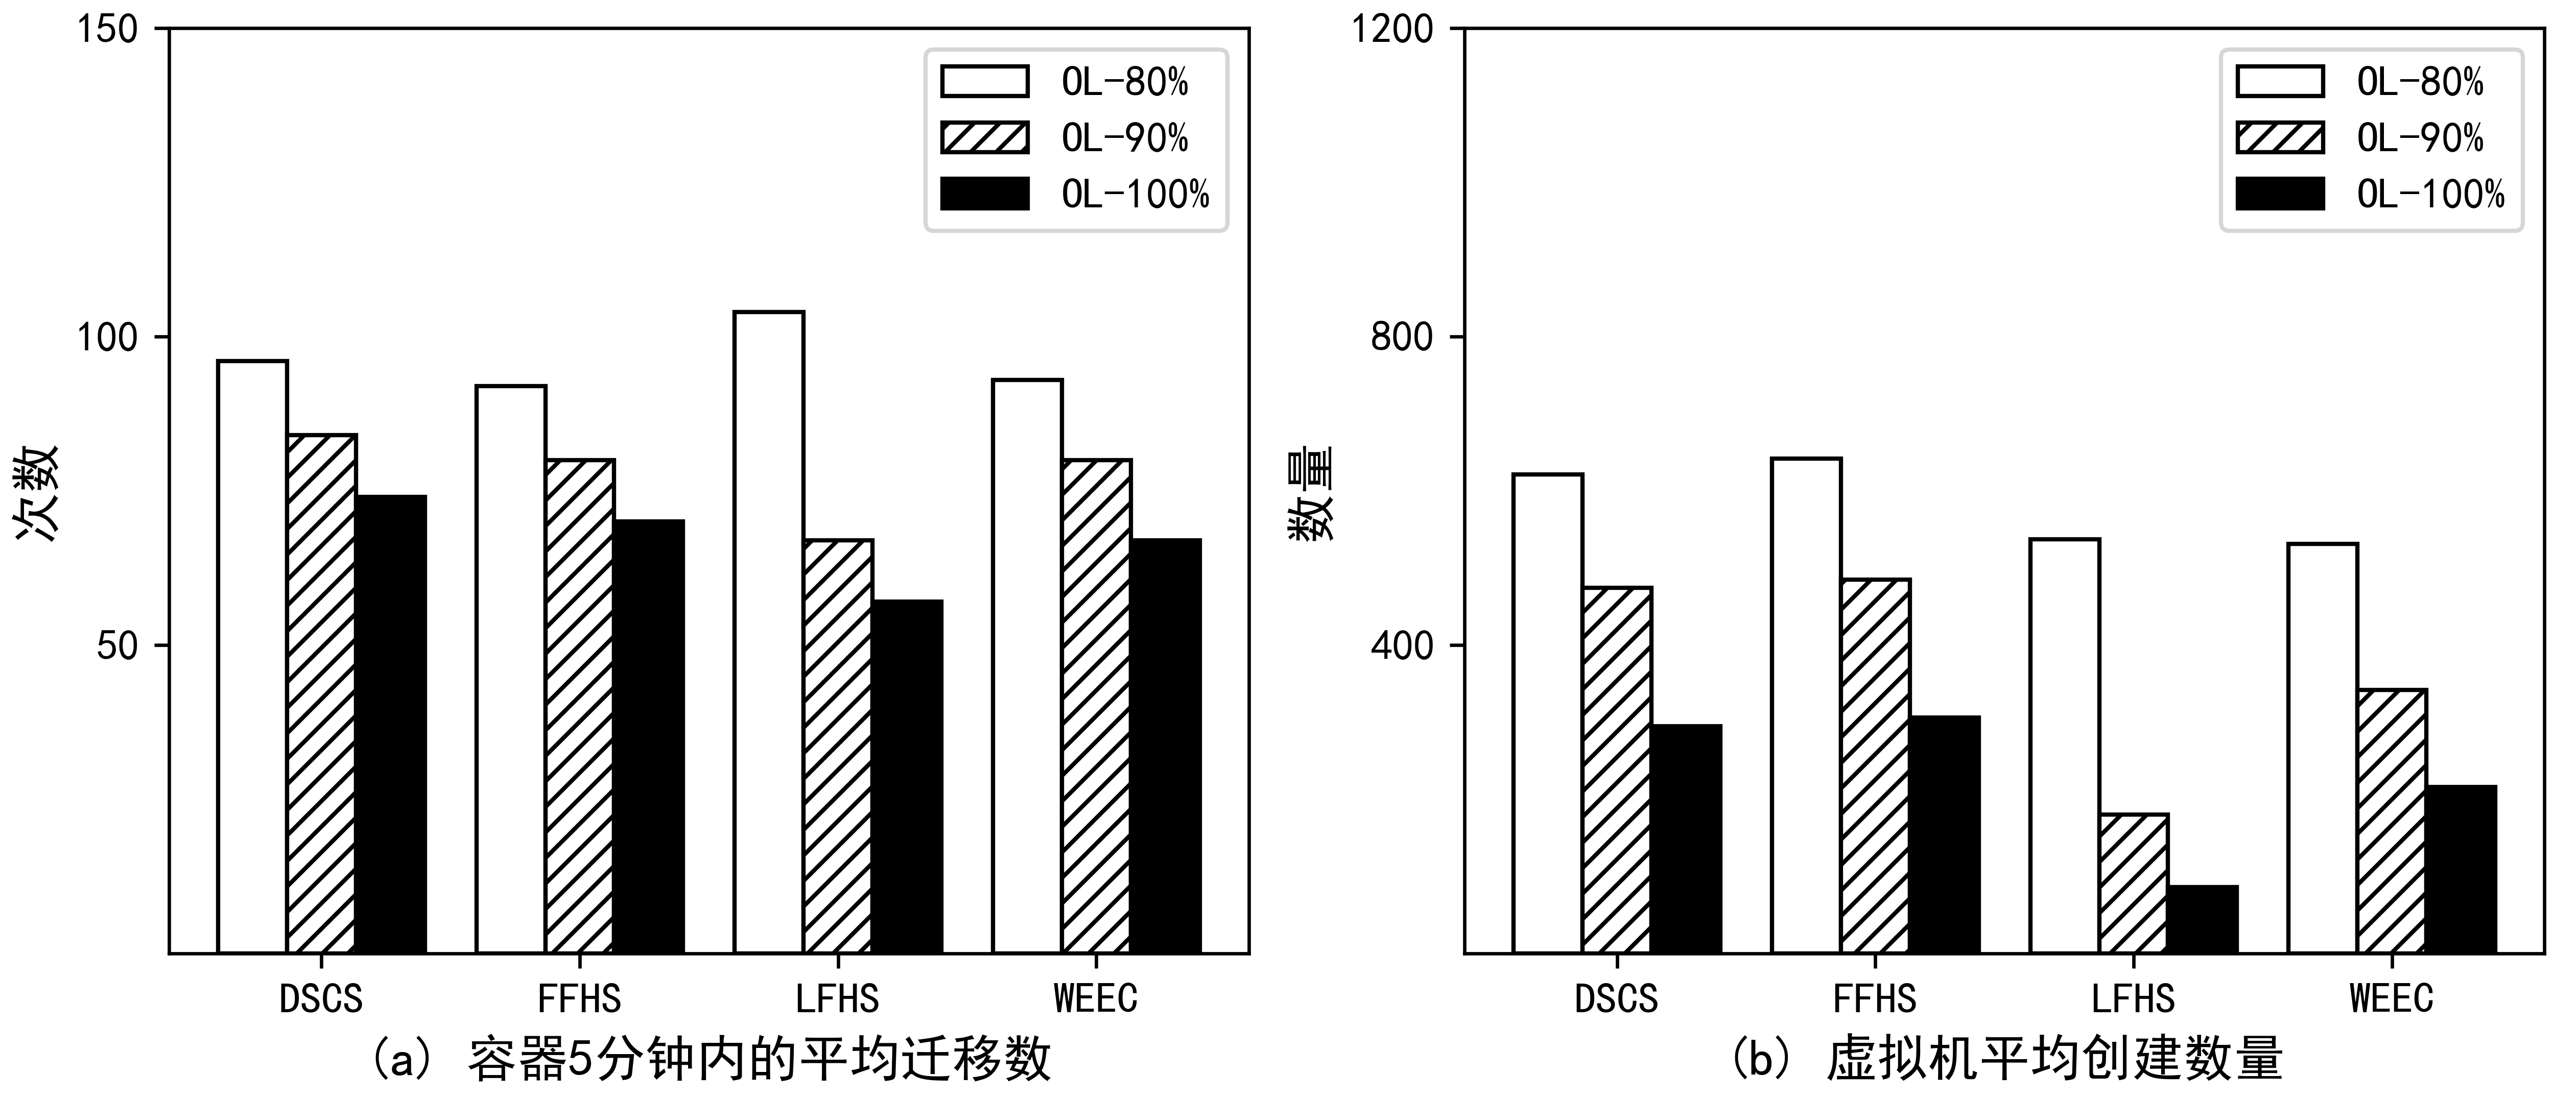
\includegraphics[width=0.45\textwidth]{figures/fig15_4-4_a.png}
    \end{figure}
\end{minipage}
\begin{minipage}{\textwidth}
    \centering
    \begin{figure}[htb]
    \centering
    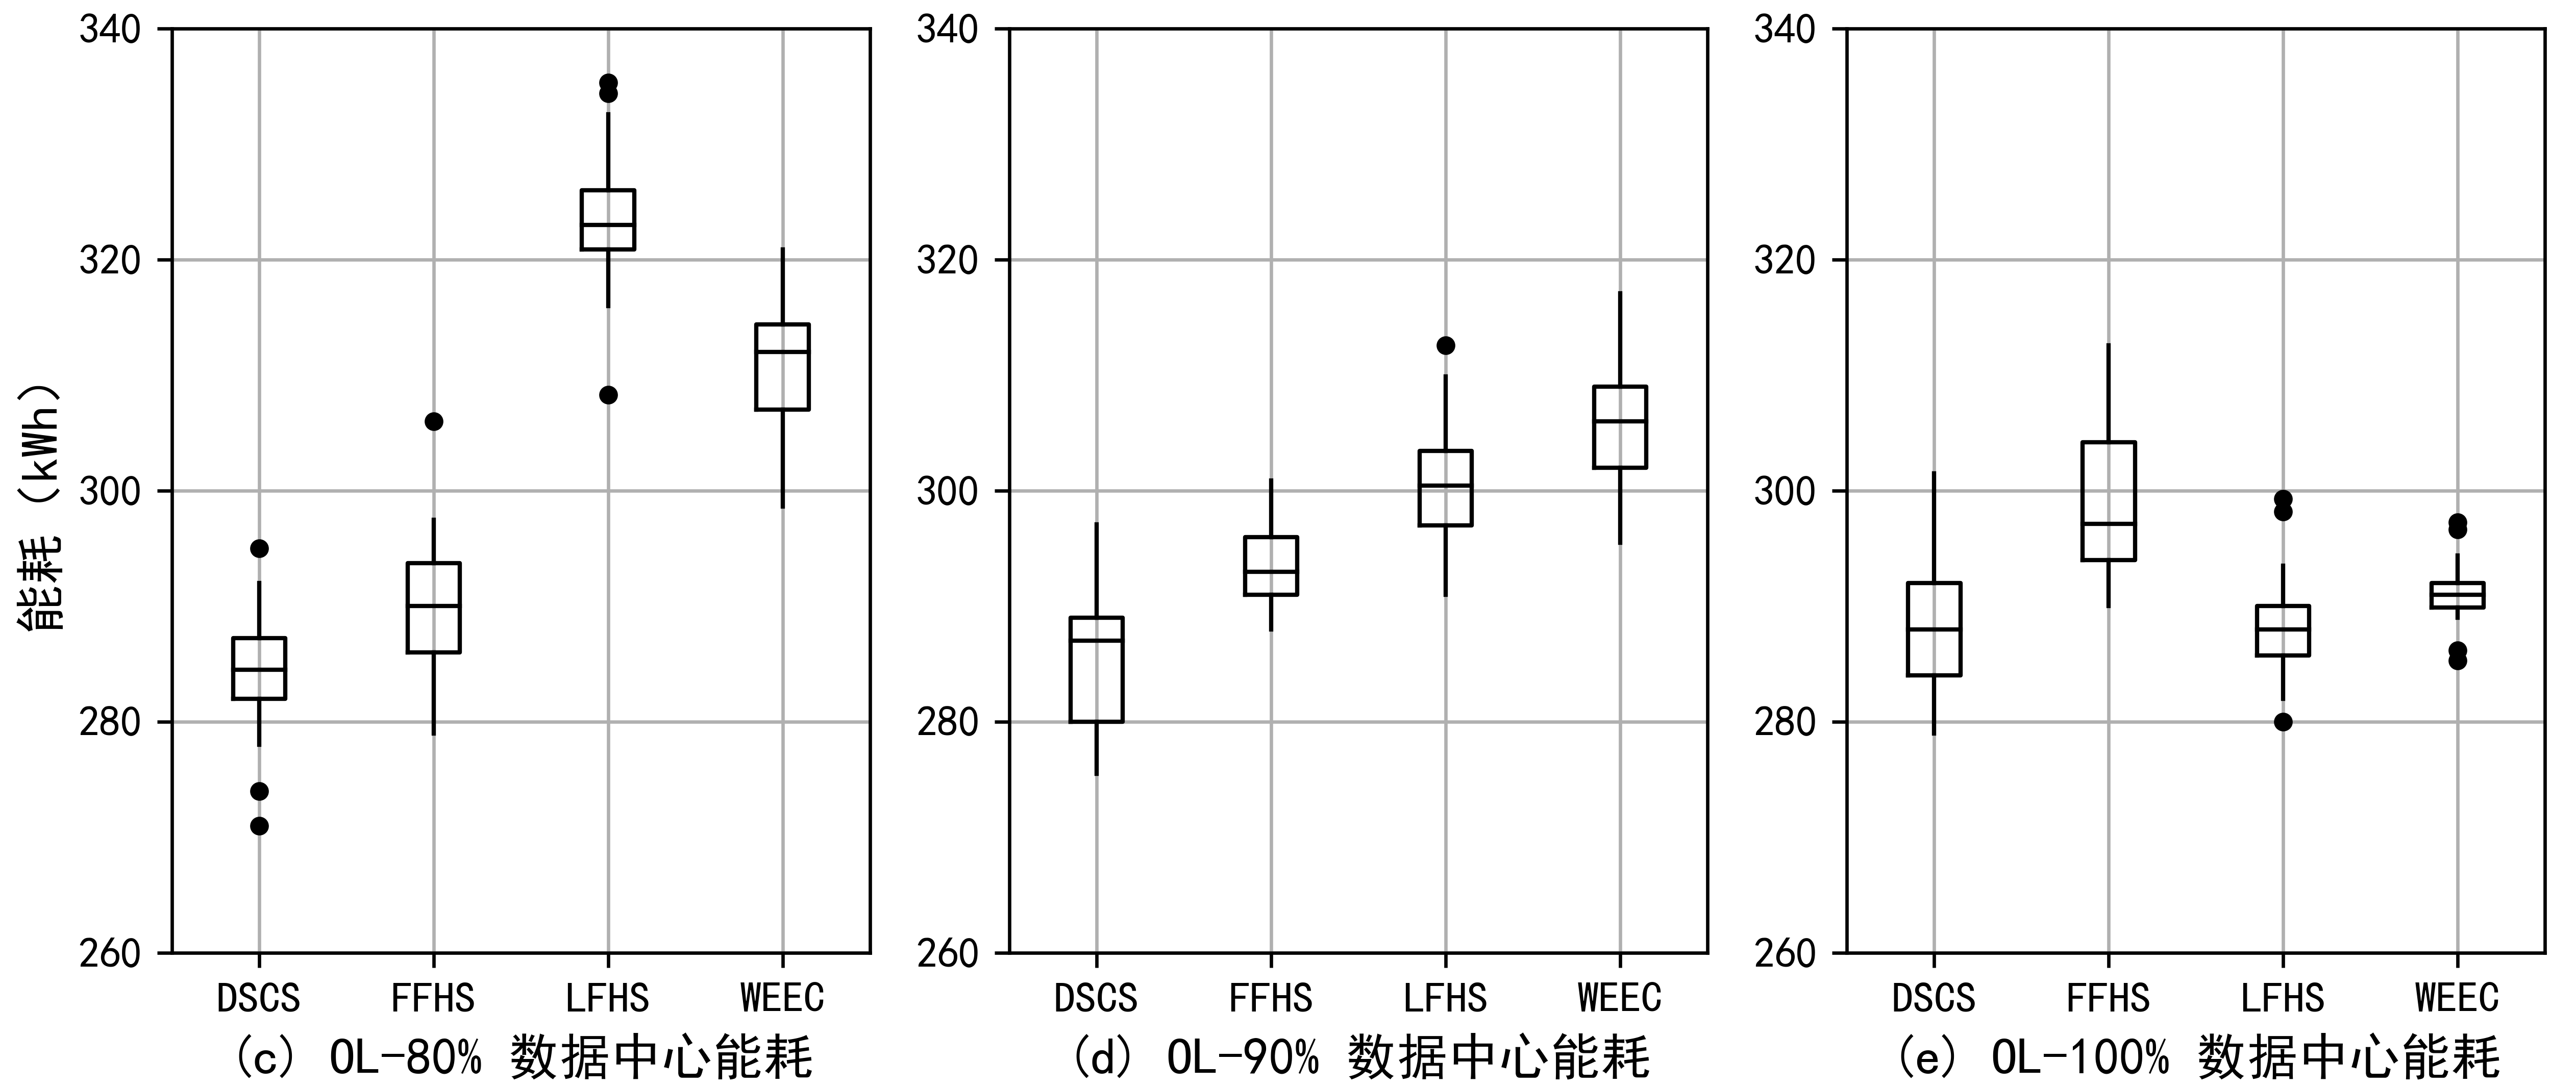
\includegraphics[width=0.45\textwidth]{figures/fig15_4-4_b.png}
    \end{figure}
\end{minipage}
\begin{minipage}{\textwidth}
    \centering
    \begin{figure}[htb]
    \centering
    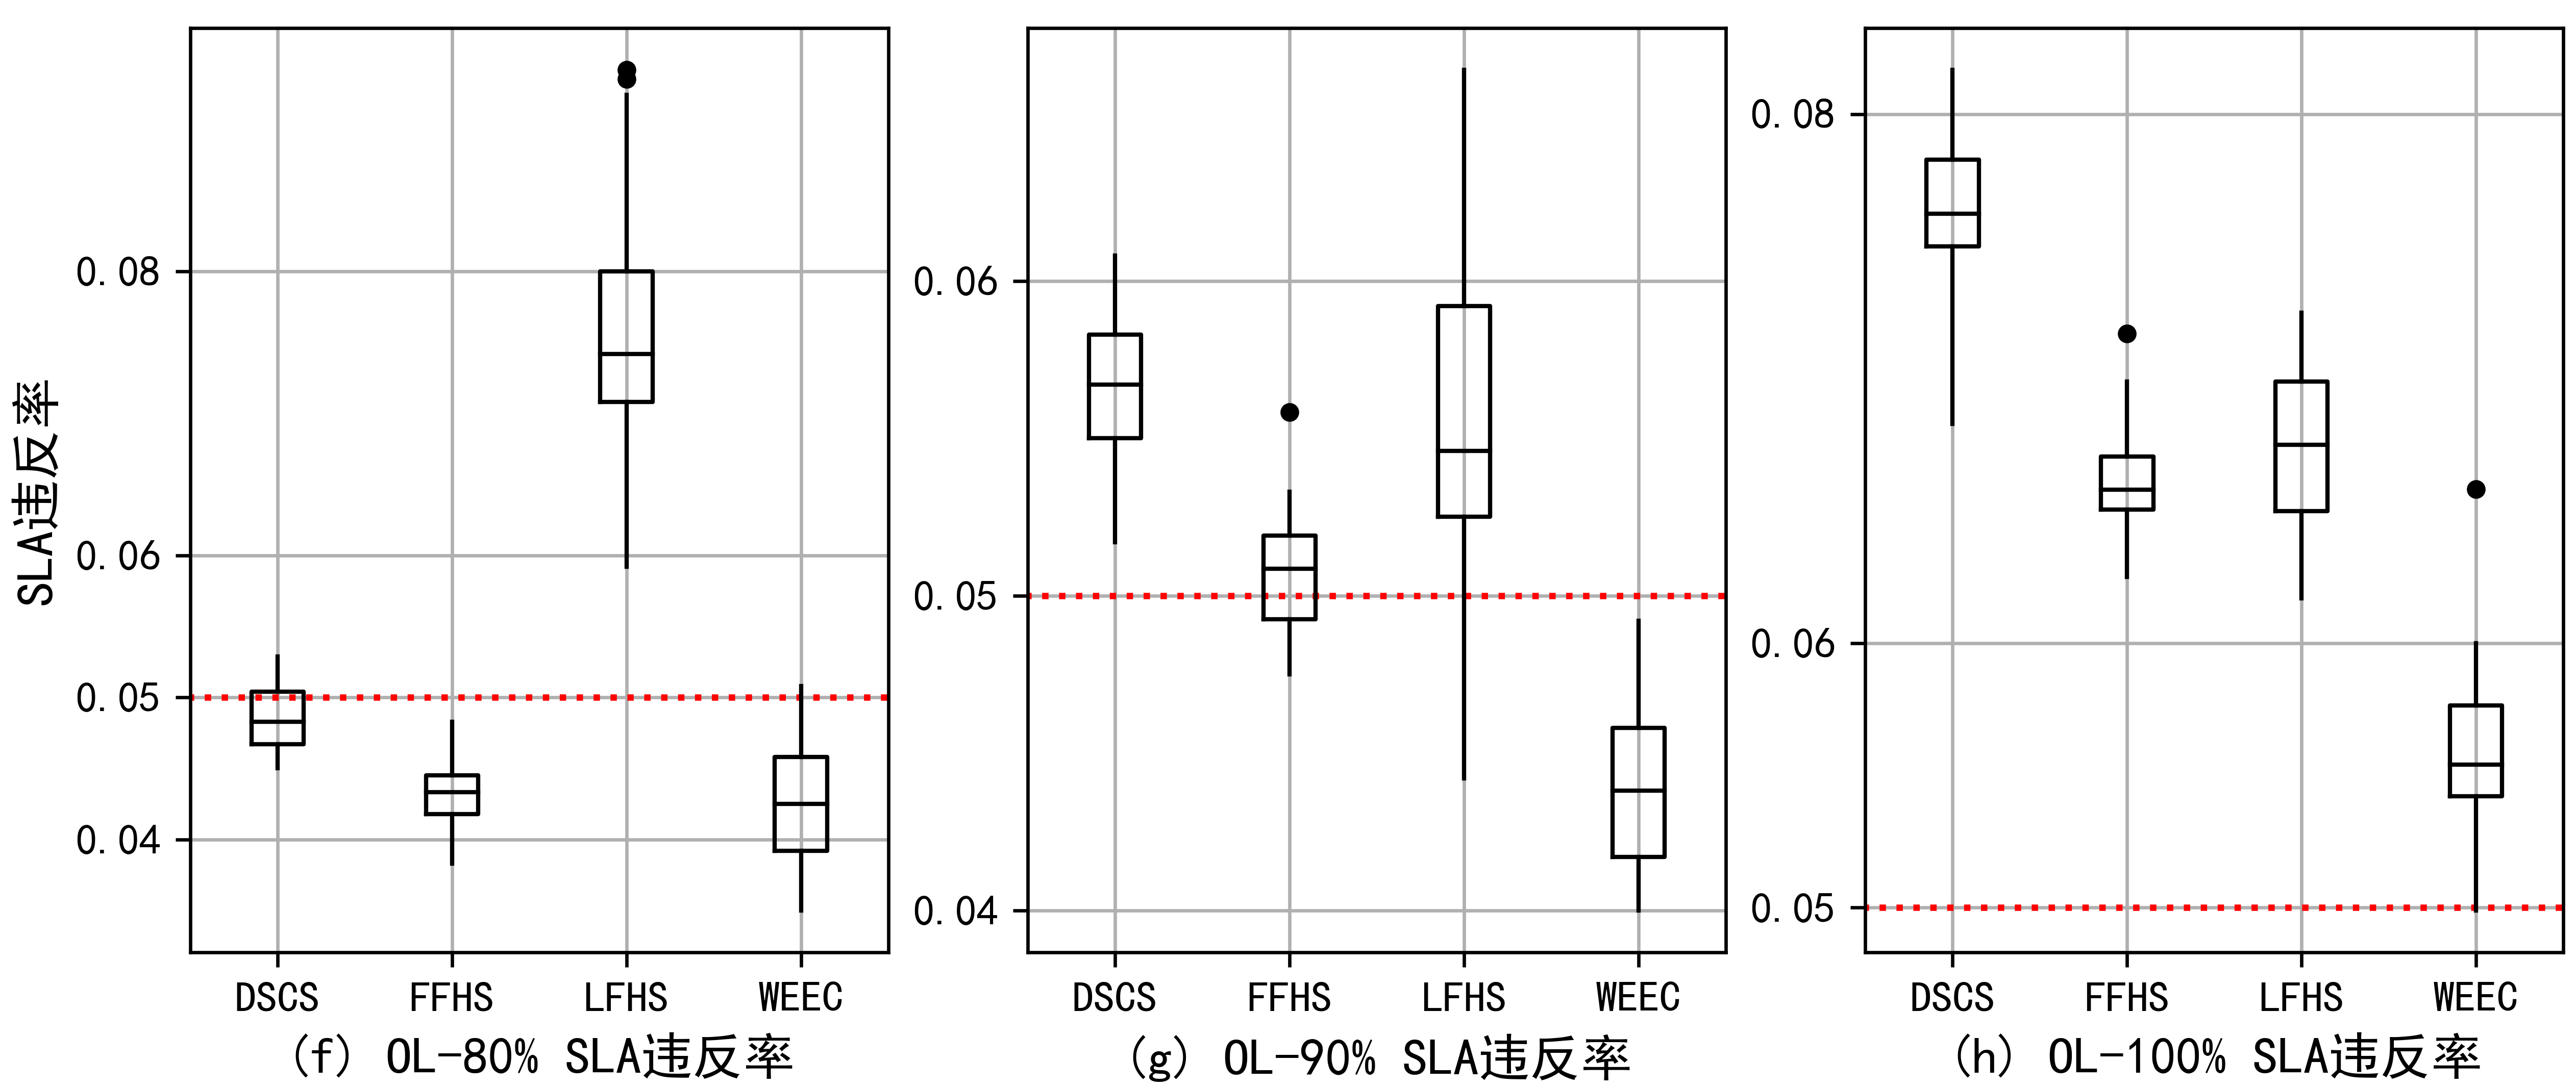
\includegraphics[width=0.45\textwidth]{figures/fig15_4-4_c.png}
    \caption{group.1 4种调度策略容器迁移、虚拟机创建数、能耗和SLA对比}
    \label{fig:fig15}
    \end{figure}
\end{minipage}
\end{frame}

\begin{frame}
\frametitle{实验结果与分析}
\framesubtitle{实验结果:group.2 \textbf{UL=$[50\%,60\%,70\%]$ OL=$80\%$, Overbooking=$80th$}}
\begin{minipage}{\textwidth}
    \centering
    \begin{figure}[htb]
    \centering
    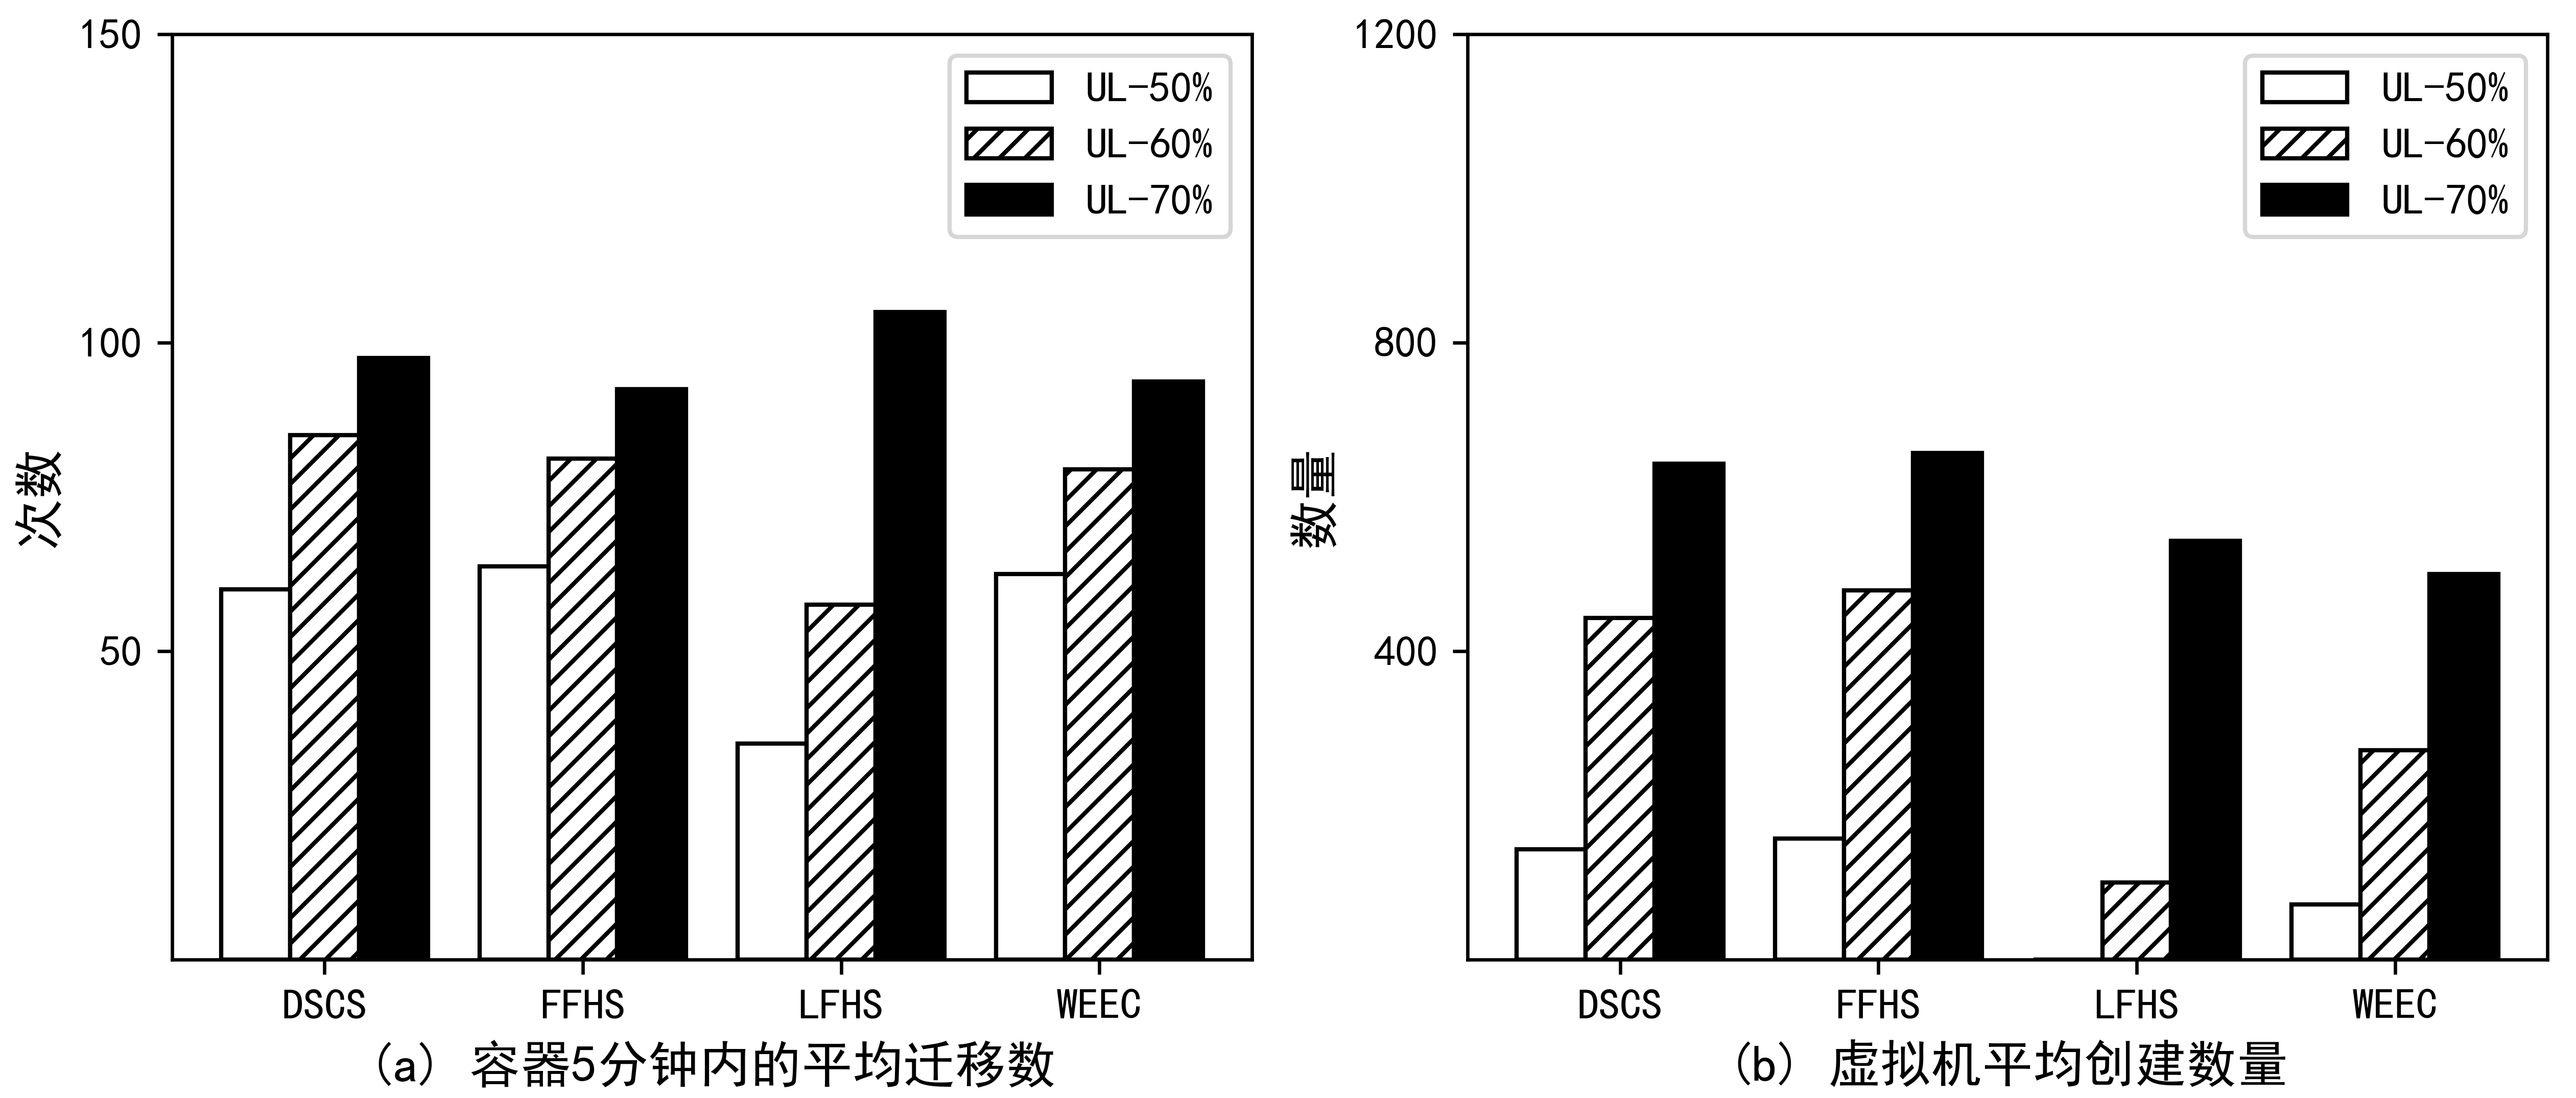
\includegraphics[width=0.45\textwidth]{figures/fig16_4-5_a.png}
    \end{figure}
\end{minipage}
\begin{minipage}{\textwidth}
    \centering
    \begin{figure}[htb]
    \centering
    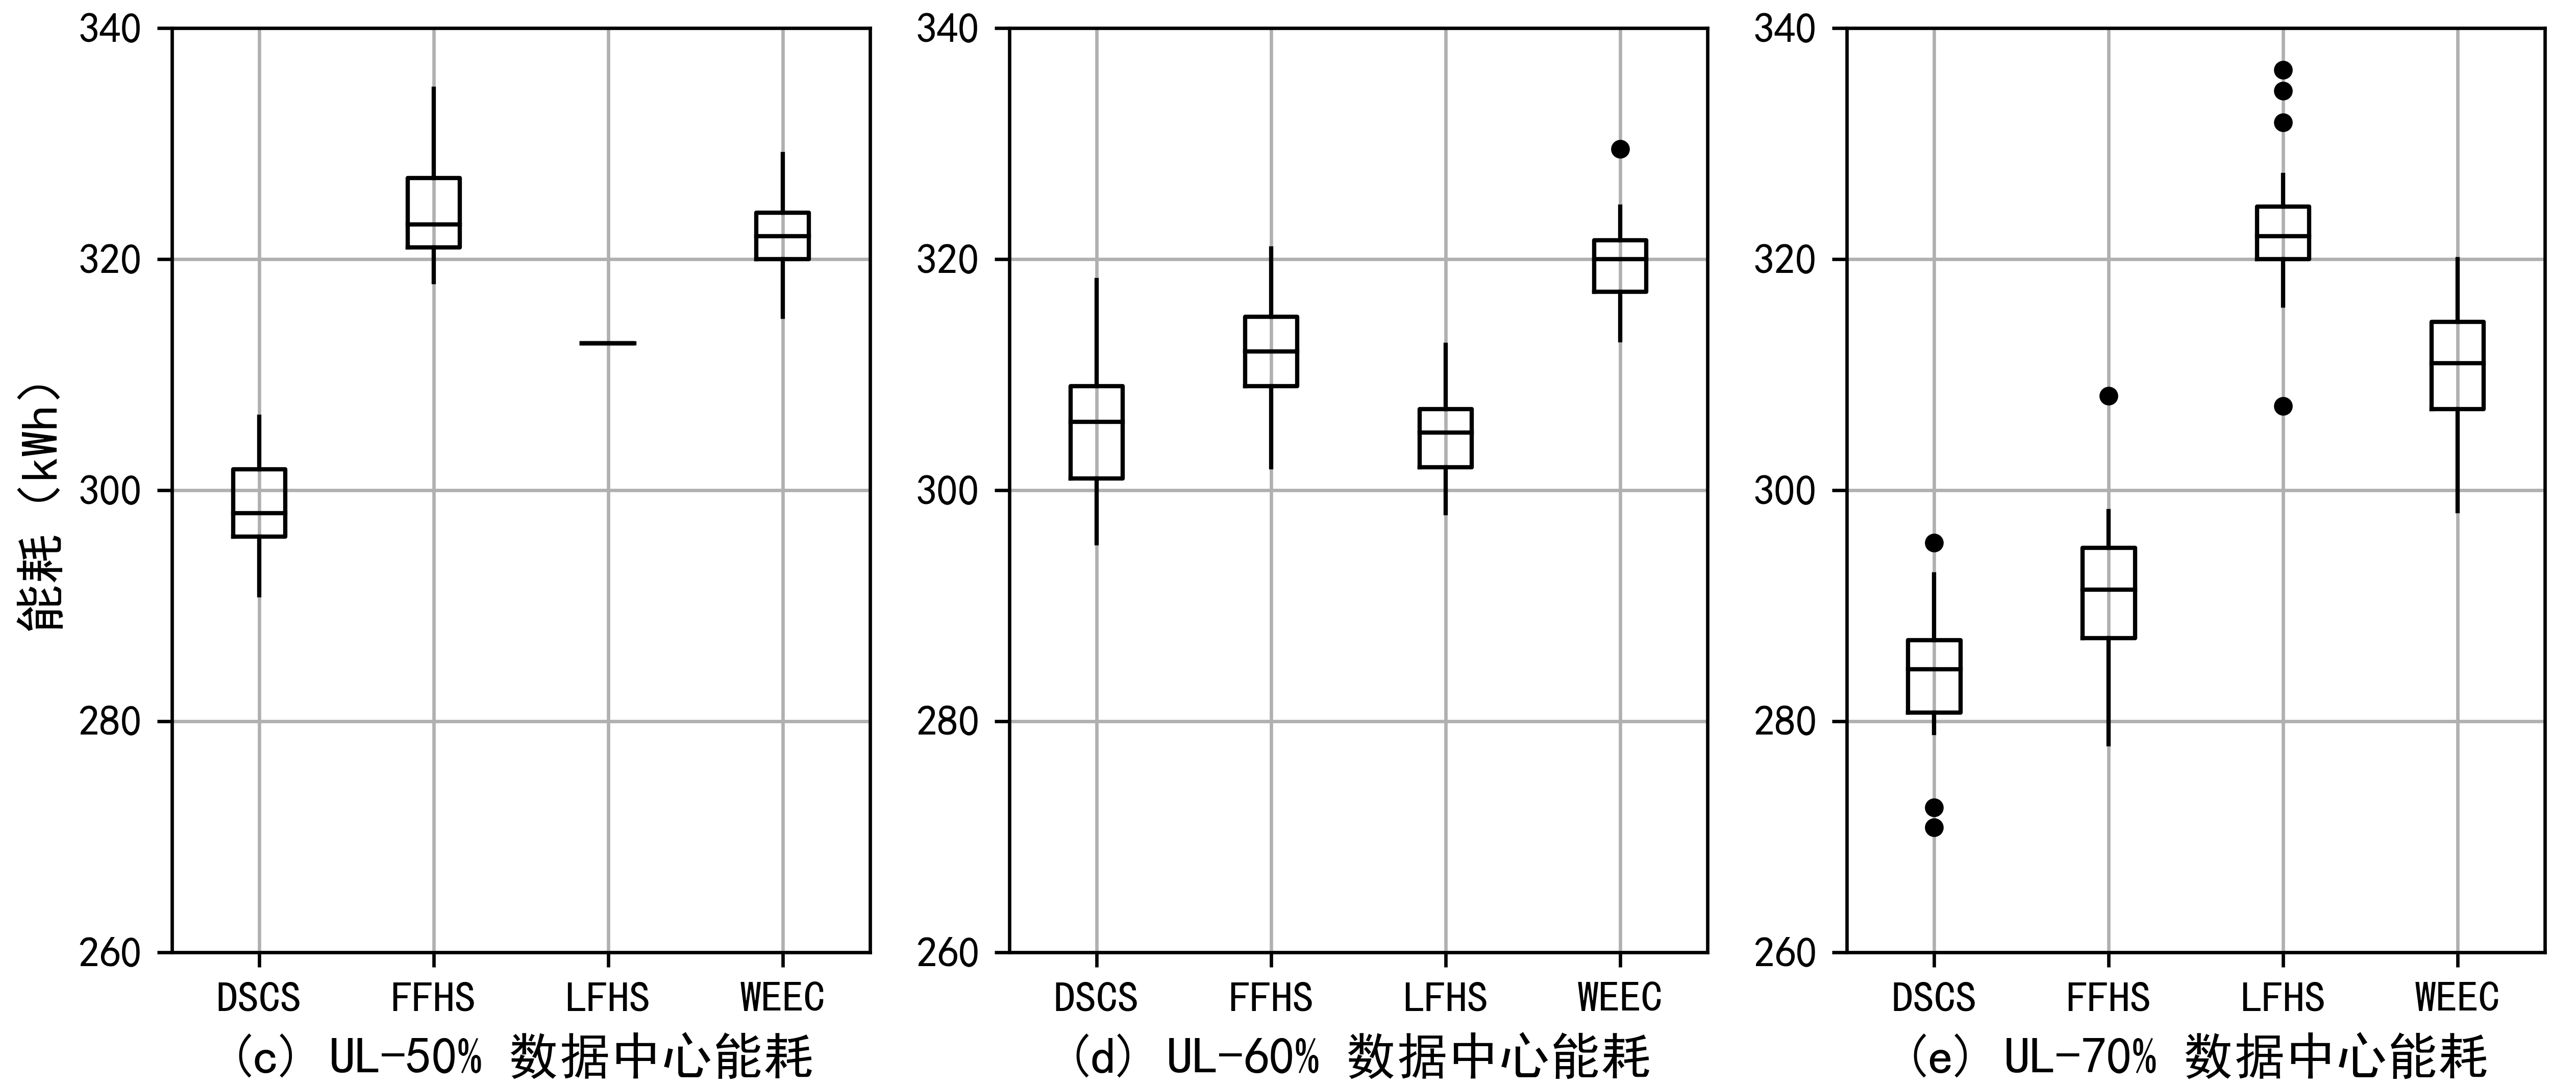
\includegraphics[width=0.45\textwidth]{figures/fig16_4-5_b.png}
    \end{figure}
\end{minipage}
\begin{minipage}{\textwidth}
    \centering
    \begin{figure}[htb]
    \centering
    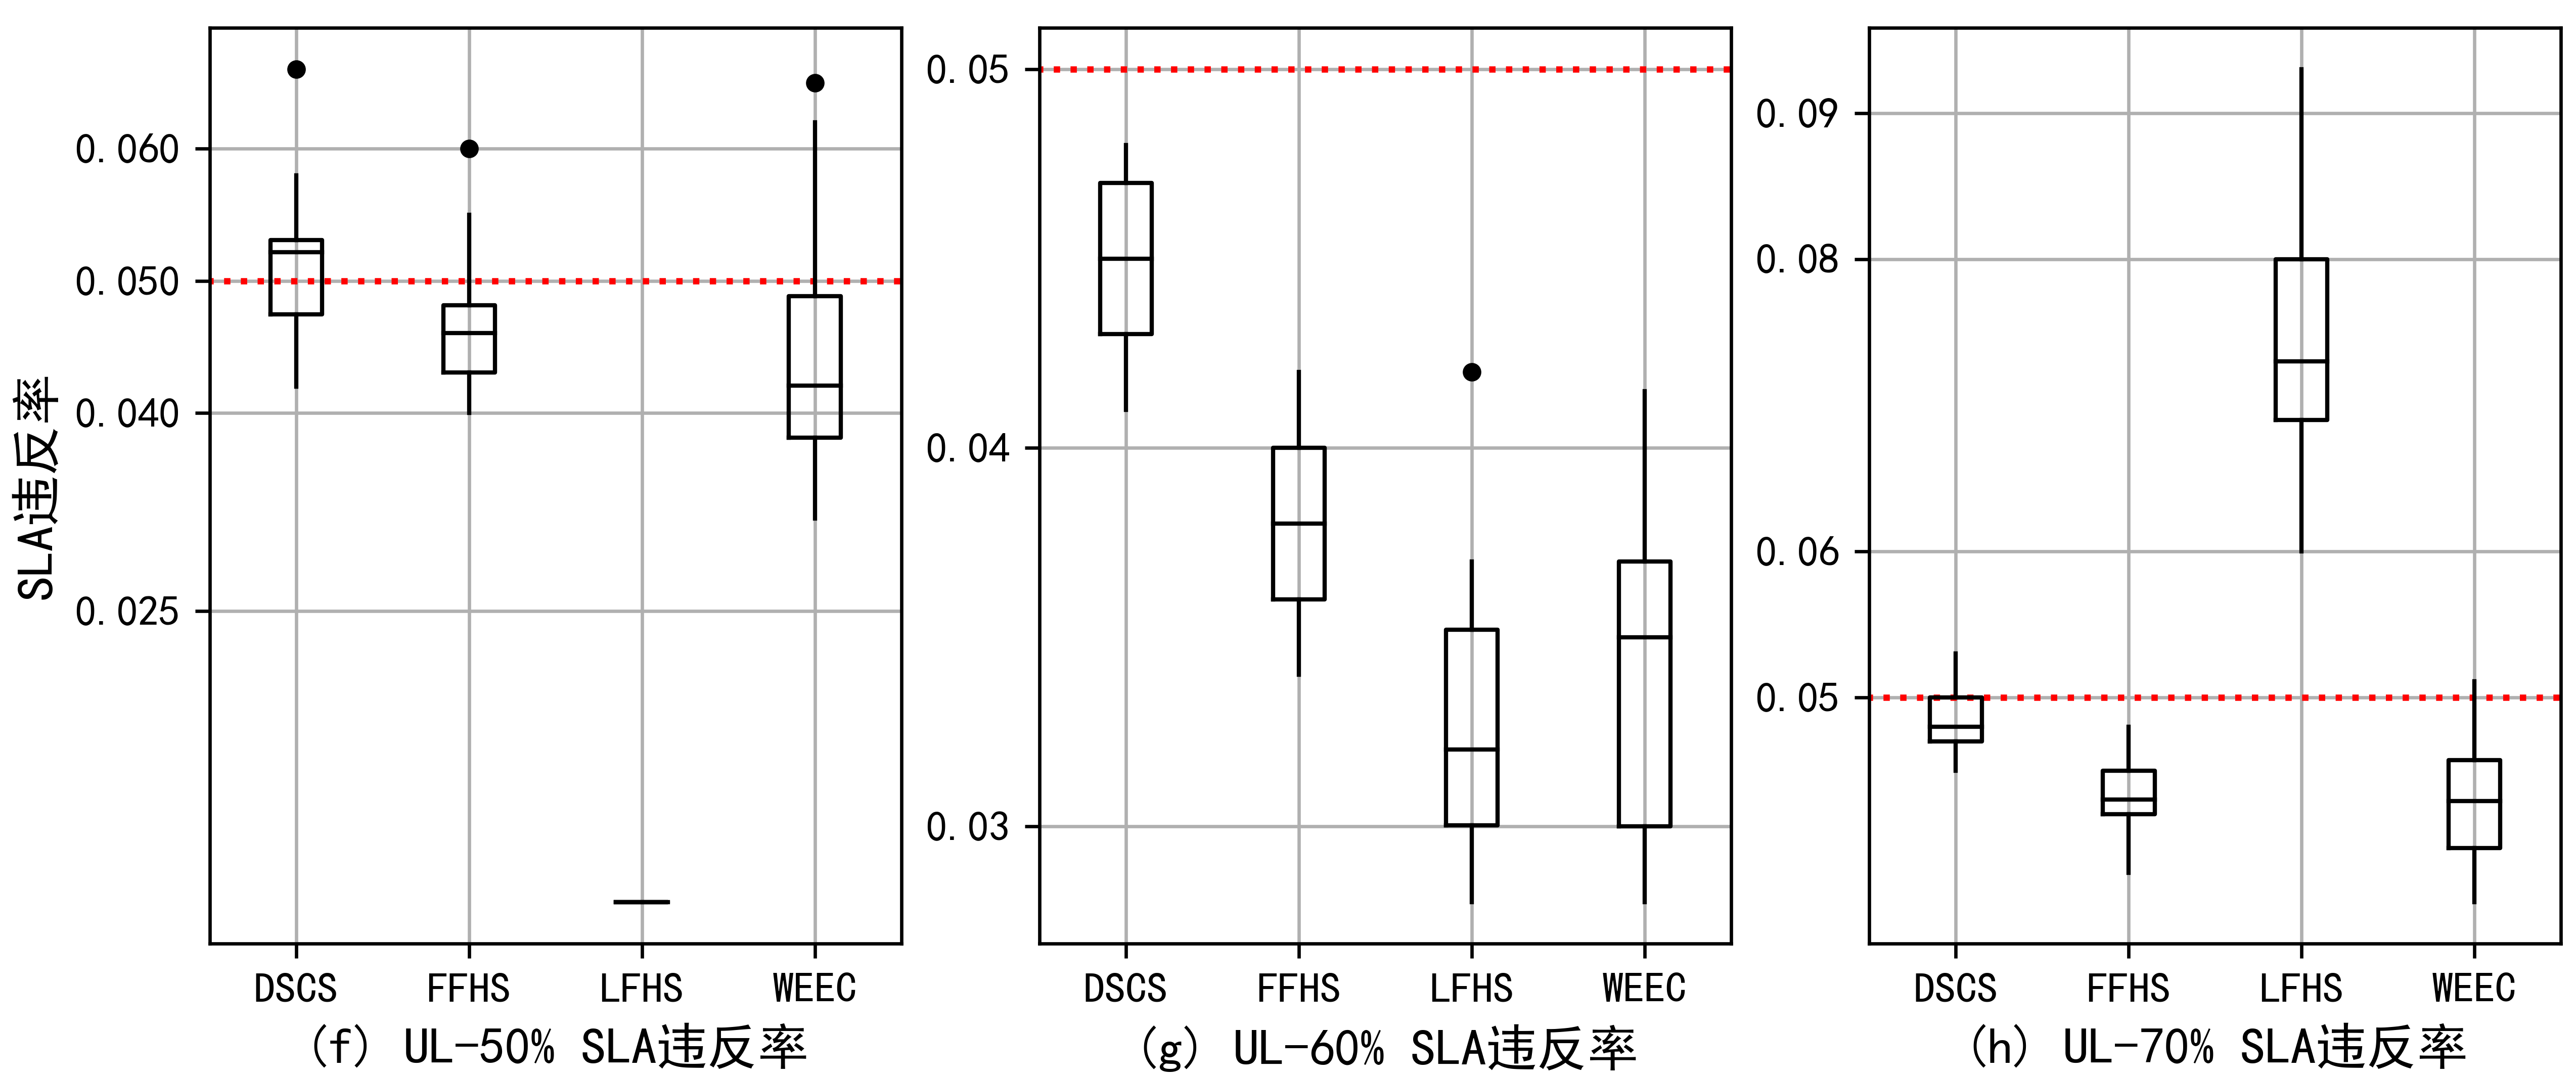
\includegraphics[width=0.45\textwidth]{figures/fig16_4-5_c.png}
    \caption{group.2 4种调度策略容器迁移、虚拟机创建数、能耗和SLA对比}
    \label{fig:fig16}
    \end{figure}
\end{minipage}
\end{frame}

\begin{frame}
\frametitle{实验结果与分析}
\framesubtitle{实验结果:group.3 \textbf{UL=$70\%$ OL=$80\%$, Overbooking=$[20th,40th,80th]$}}
\begin{minipage}{\textwidth}
    \centering
    \begin{figure}[htb]
    \centering
    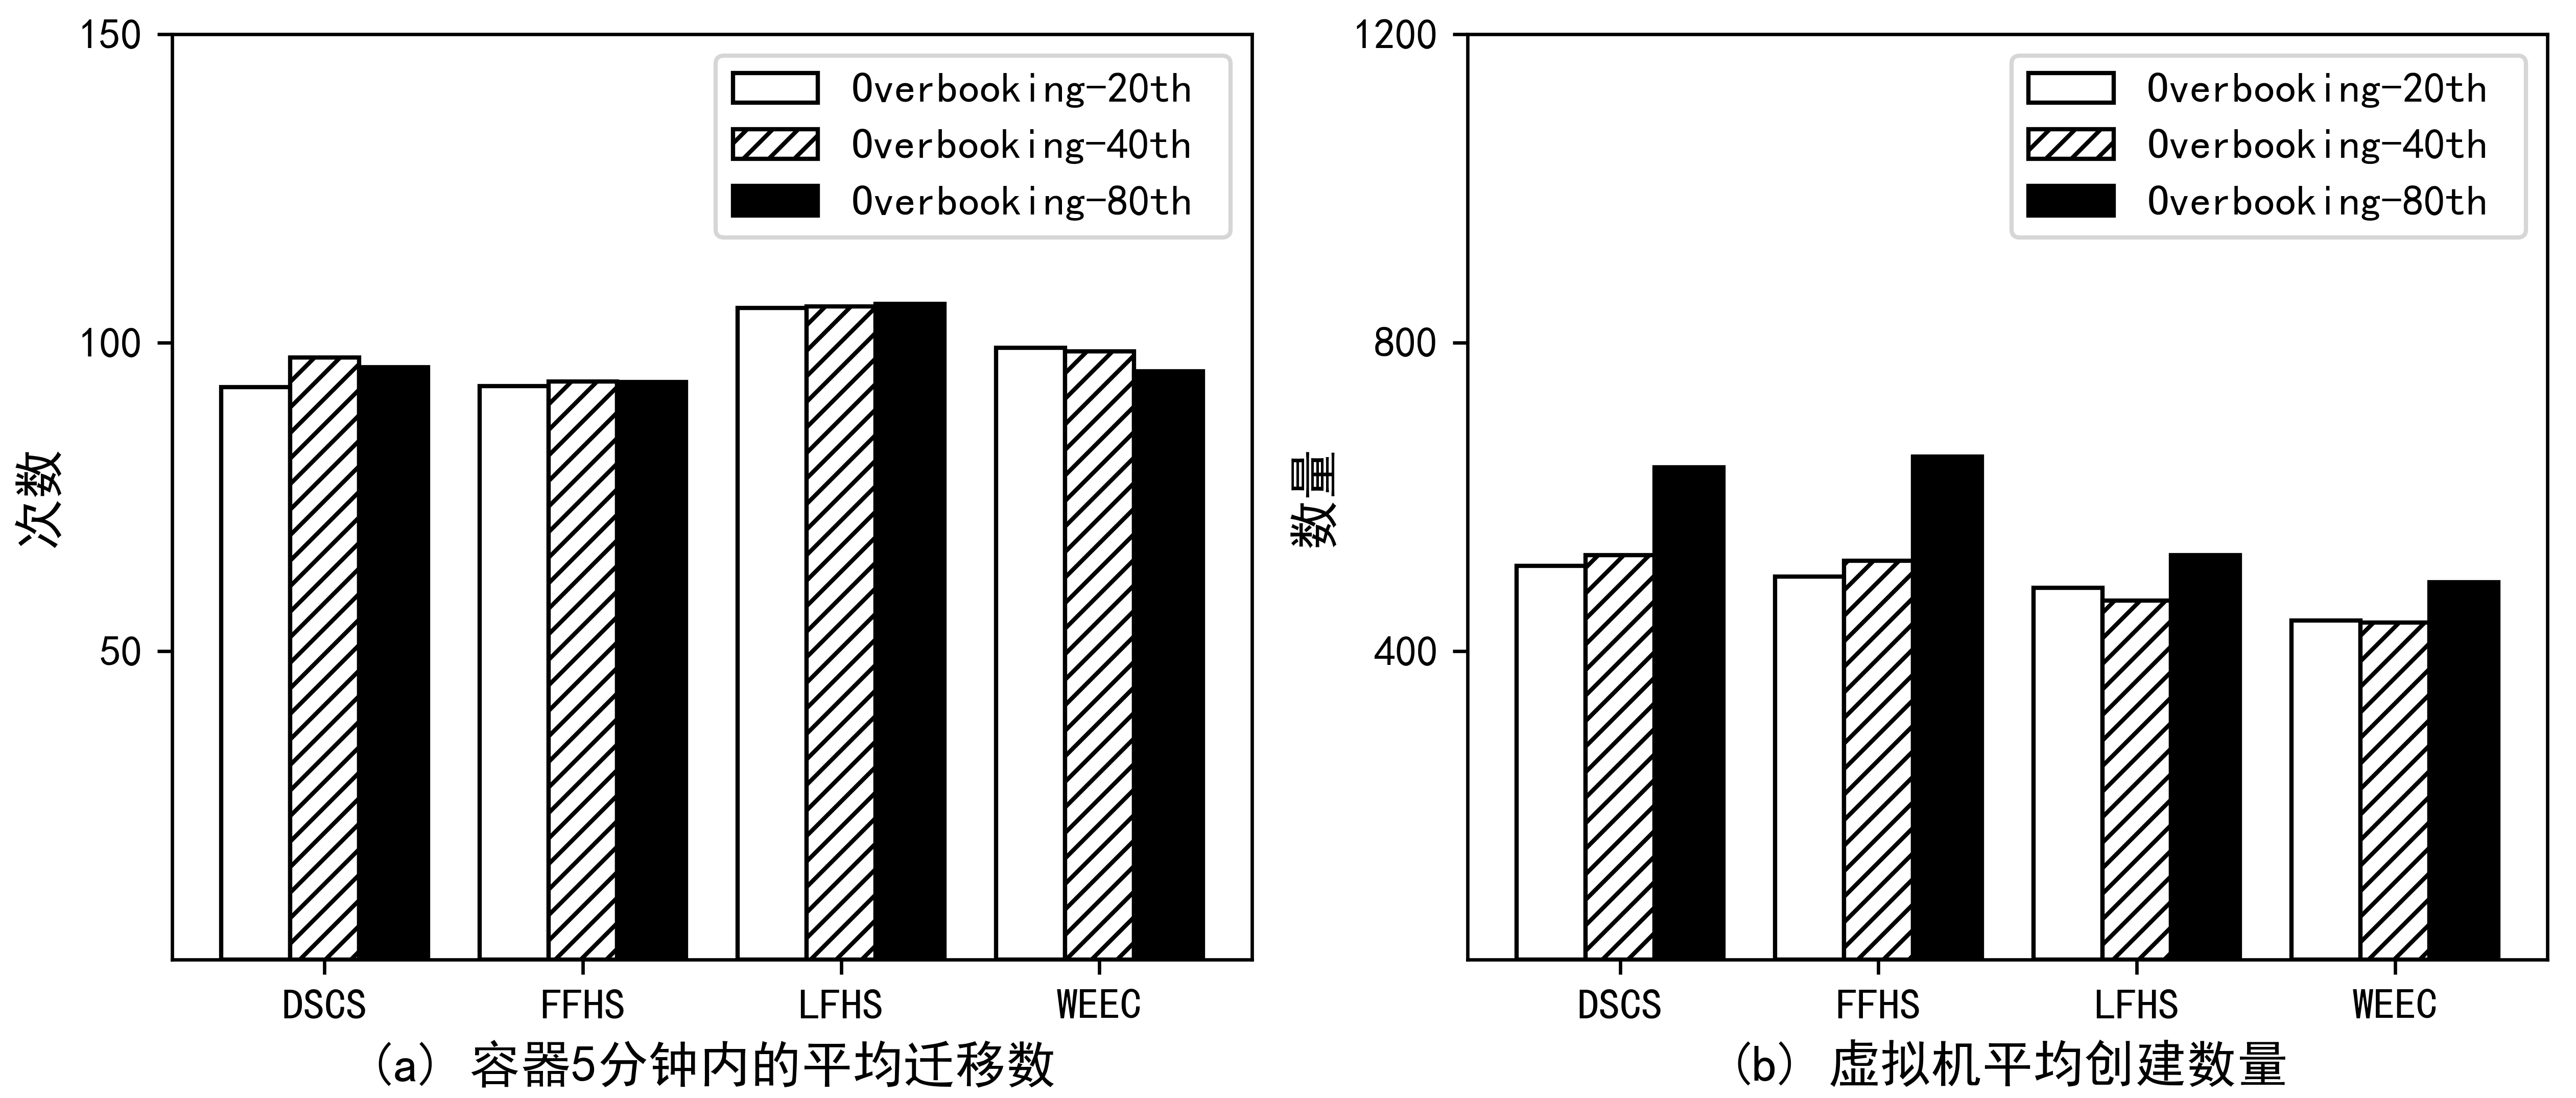
\includegraphics[width=0.45\textwidth]{figures/fig17_4-6_a.png}
    \end{figure}
\end{minipage}
\begin{minipage}{\textwidth}
    \centering
    \begin{figure}[htb]
    \centering
    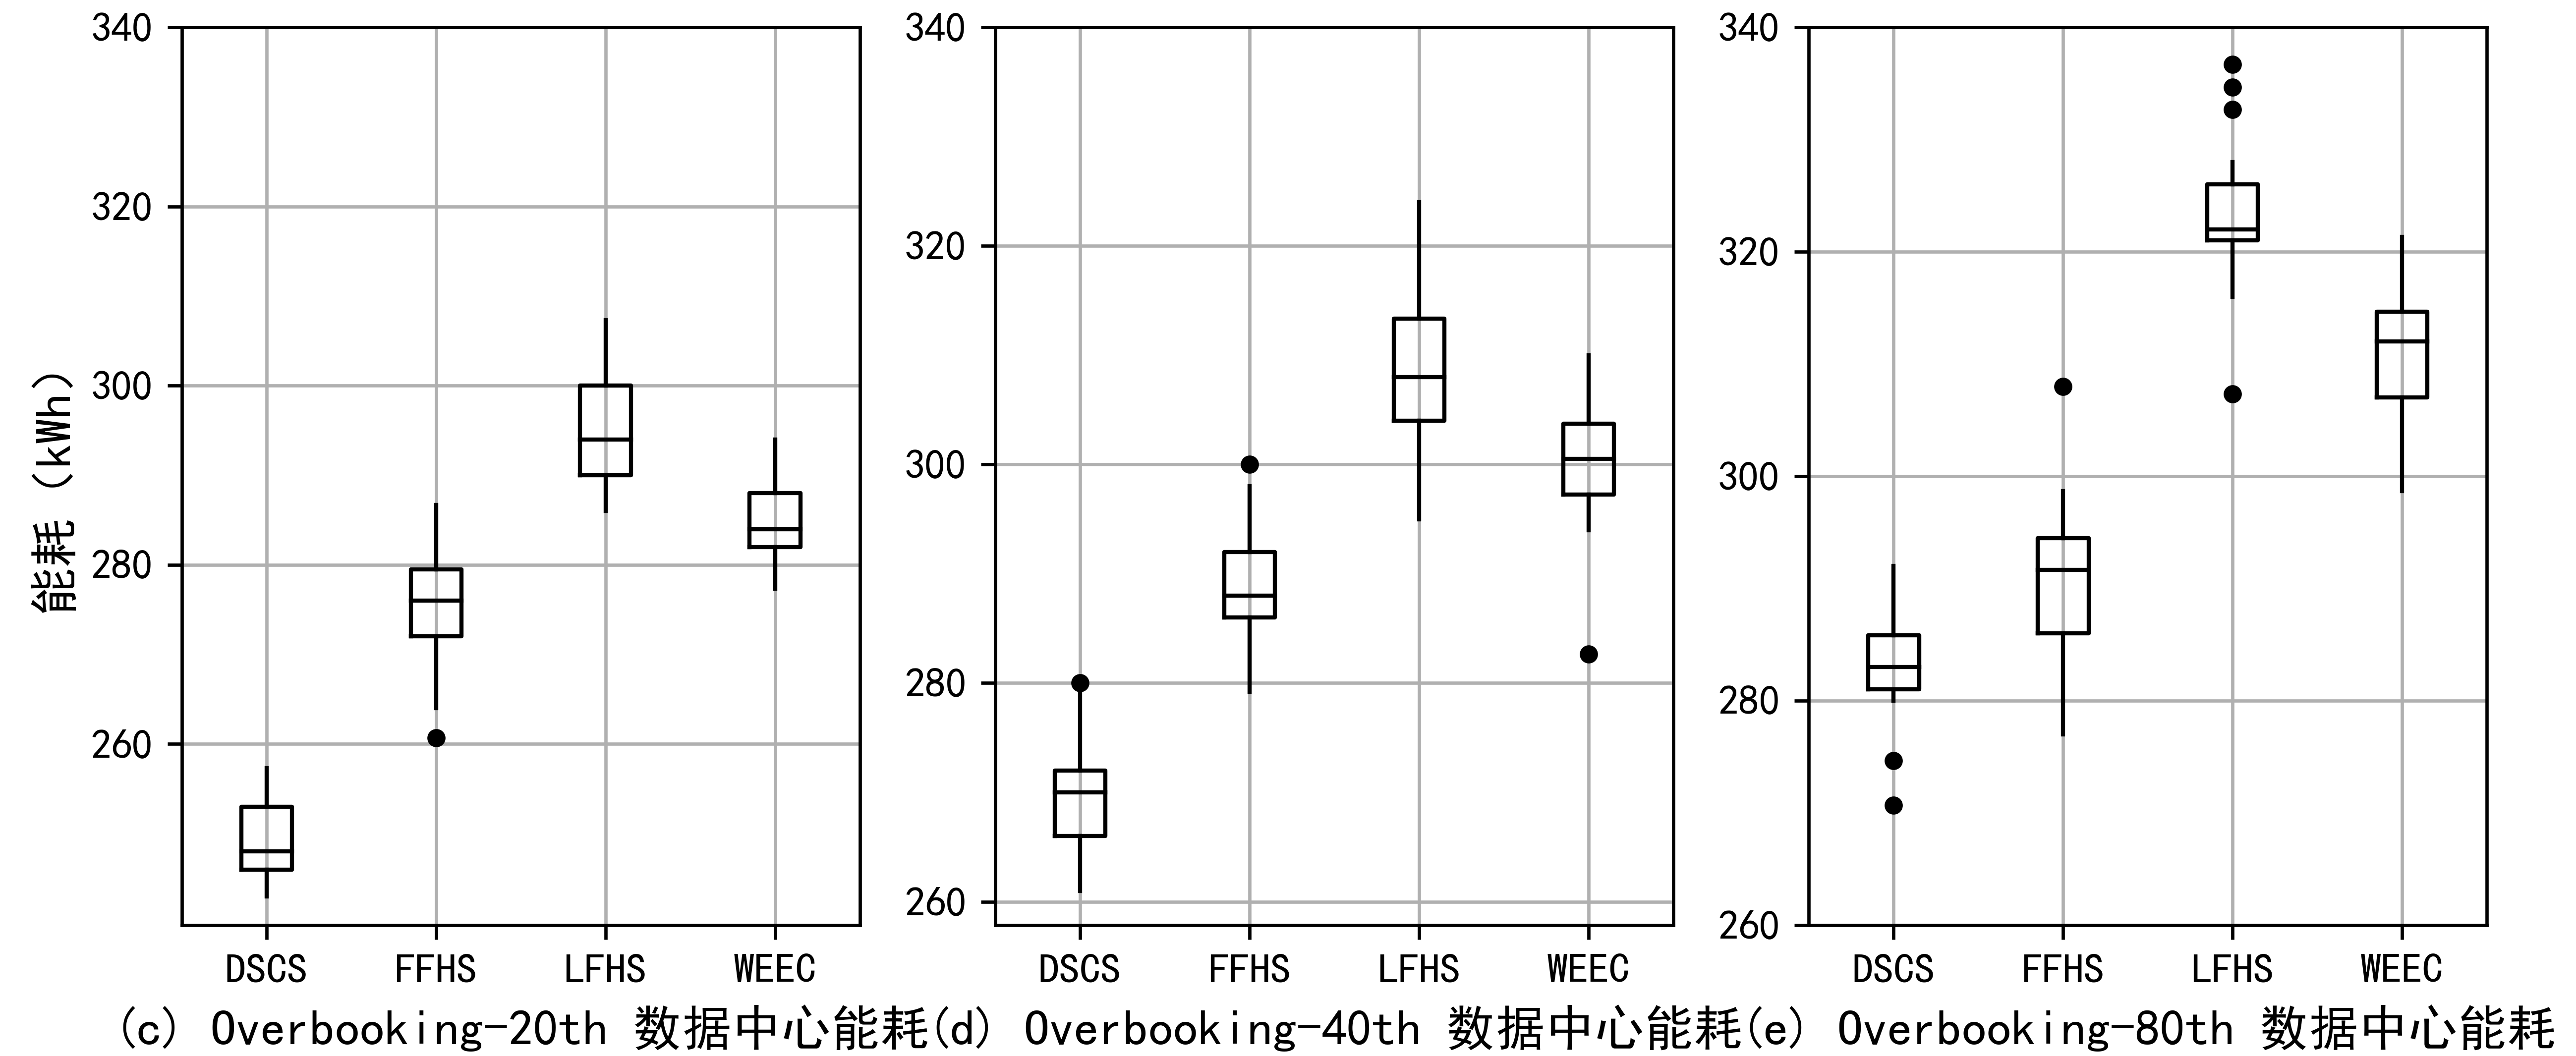
\includegraphics[width=0.45\textwidth]{figures/fig17_4-6_b.png}
    \end{figure}
\end{minipage}
\begin{minipage}{\textwidth}
    \centering
    \begin{figure}[htb]
    \centering
    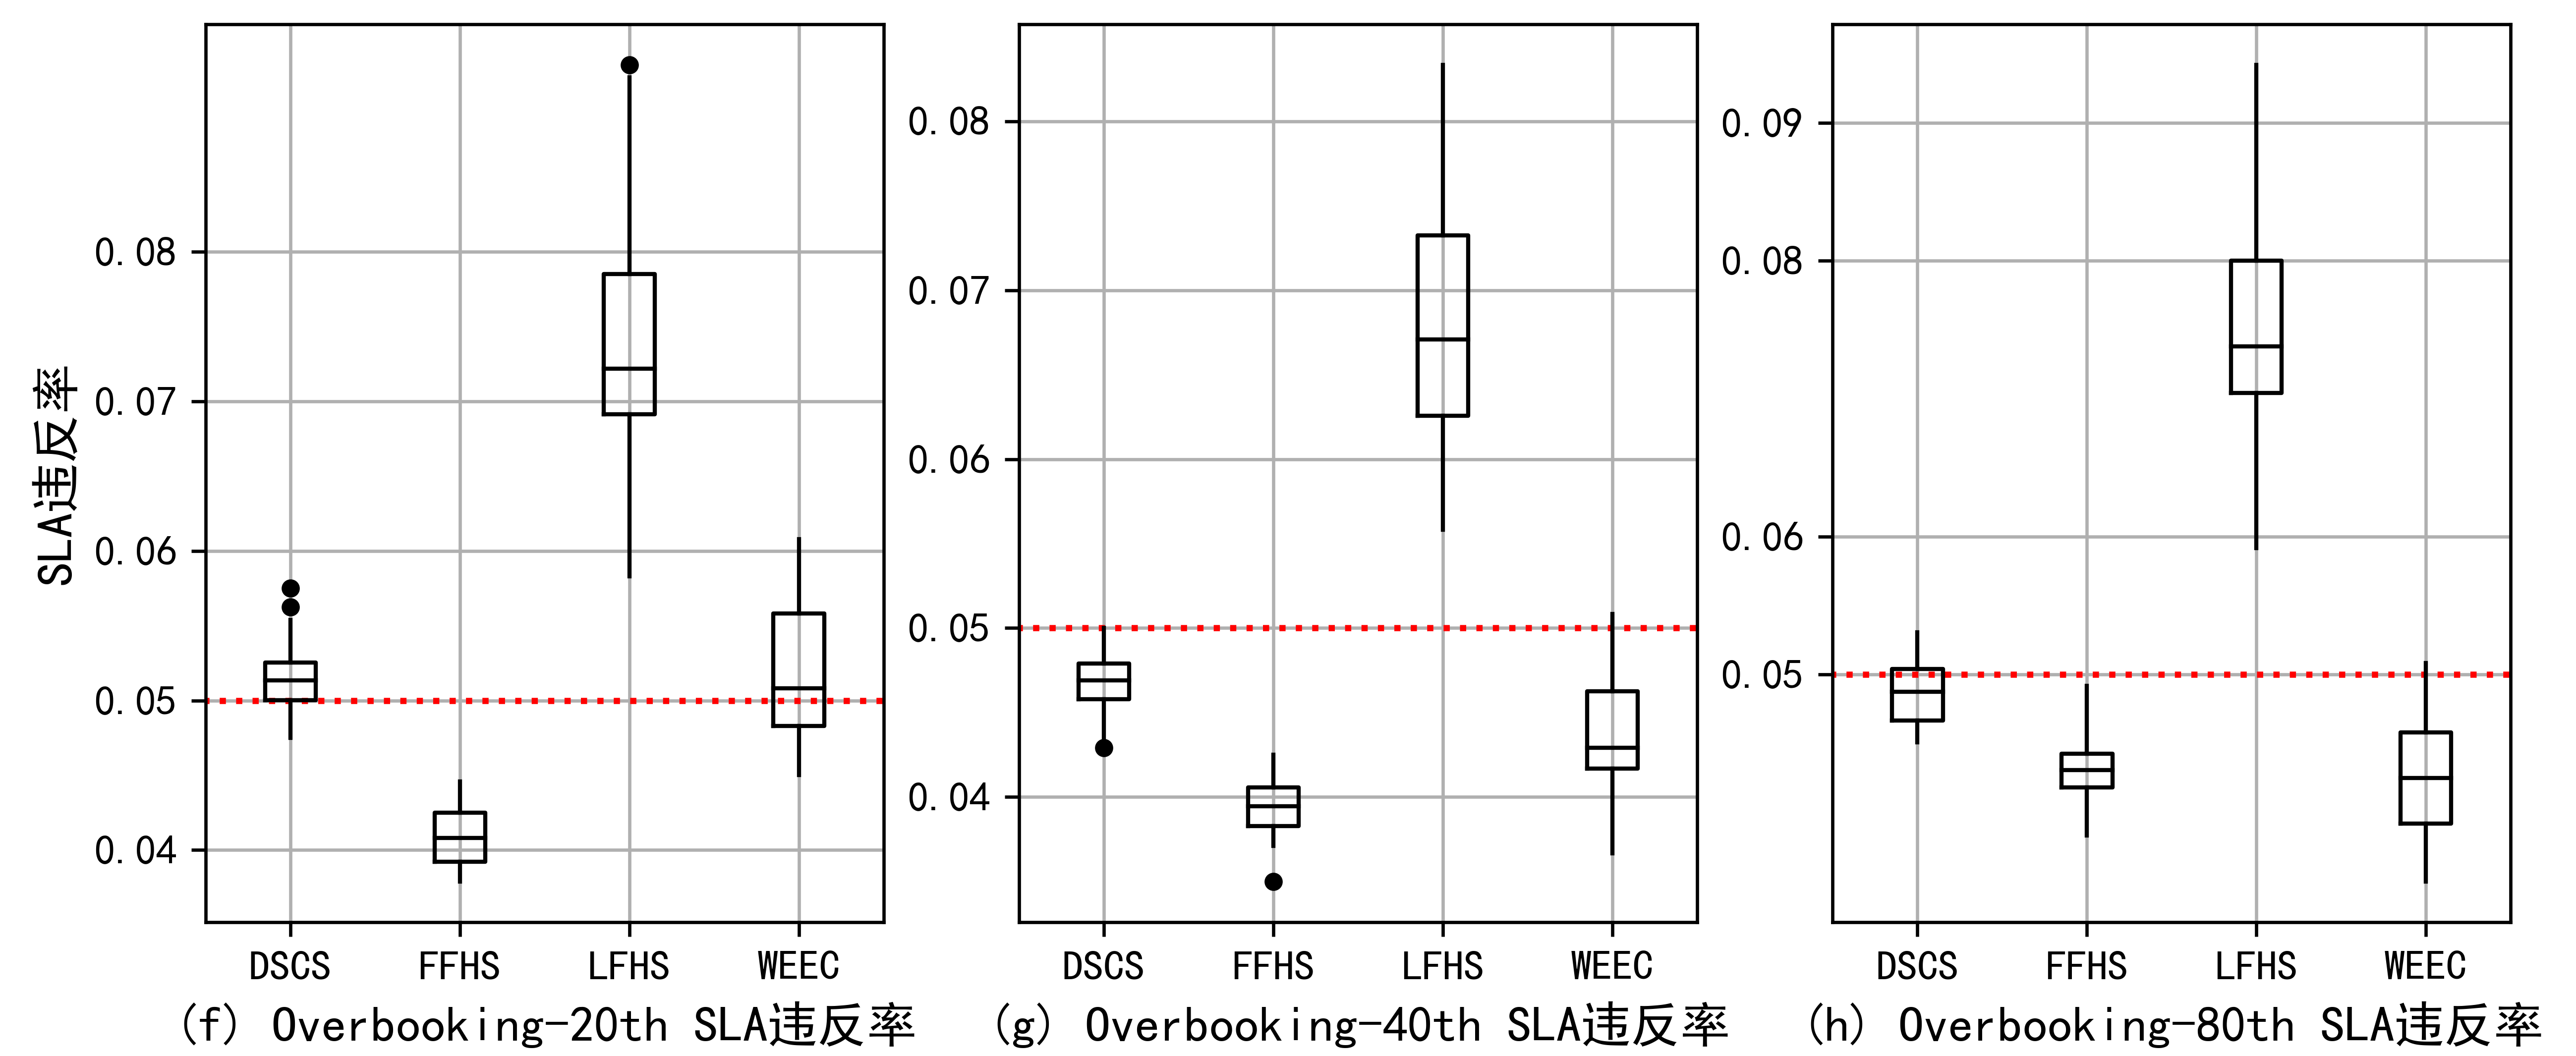
\includegraphics[width=0.45\textwidth]{figures/fig17_4-6_c.png}
    \caption{group.3 4种调度策略容器迁移、虚拟机创建数、能耗和SLA对比}
    \label{fig:fig17}
    \end{figure}
\end{minipage}
\end{frame}

\begin{frame}
\frametitle{实验结果与分析}
\framesubtitle{SLA违反补偿协议}
\begin{itemize}
    \item 主流云服务商(GCP\footnote{\tiny{https://cloud.google.com/}},
    AWS\footnote{\tiny{https://aws.amazon.com/}},阿里云\footnote{\tiny{https://cn.aliyun.com/}})SLA违反补偿协议
\end{itemize}
\begin{table}[hftb]
        \centering
        \resizebox{0.8\textwidth}{!}{%
            \begin{tabular}{ccccc}
                \toprule
                \textbf{赔偿(相对于租金比例)} & \textbf{SLA违反率(未响应时间占比)} \\
                \midrule
                $0$ & $0\sim5\%$   \\
                $5$ & $5\%\sim15\%$   \\
                $10$ & $15\%\sim20\%$   \\
                $20$ & $20\%\sim25\%$   \\
                $35$ & $25\%\sim30\%$   \\
                $55$ & $30\%\sim45\%$   \\
                $80$ & $45\%\sim50\%$   \\
                $100$ & $50\%$以上   \\
                \bottomrule
            \end{tabular}
        }
        \caption{主流云供应商SLA违反补偿金计算}
        \label{tab:tab6}
    \end{table}
\end{frame}